\documentclass[11pt,a4paper]{article}
\usepackage[utf8x]{inputenc}
\usepackage[T1]{fontenc}

\usepackage{mathptmx} 
\usepackage{float}
\usepackage{longtable}

\usepackage[pdftex]{graphicx} 
\usepackage[polish]{babel} 
\usepackage[pdftex,linkcolor=black,pdfborder={0 0 0}]{hyperref} 
\usepackage{calc} 
\usepackage{enumitem} 
\usepackage{titlesec}
\usepackage{lipsum} 
\usepackage{float}
\frenchspacing 
\linespread{1.2} 
\usepackage[a4paper, lmargin=0.1666\paperwidth, rmargin=0.1666\paperwidth, tmargin=0.1111\paperheight, bmargin=0.1111\paperheight]{geometry} 

\usepackage{enumitem}
\usepackage[all]{nowidow} 
\usepackage[protrusion=true,expansion=true]{microtype} 
\setcounter{secnumdepth}{4}

\usepackage[backend=biber]{biblatex}

\addbibresource{references-frontend.bib}

\addbibresource{references-model.bib}

\hypersetup{
    pdfsubject = {Zespołowe Przedsięwzięcie Informatyczne},
    pdftitle = {Dokumentacja ZPI Larvixon},
}

\begin{document}

\begin{titlepage}
    \centering
    {\Large \textsc{Politechnika Wrocławska} \par}
    {\large Wydział Informatyki i Telekomunikacji \par}
    {\large Kierunek: IST \par}

    \vspace{3cm}

    {\huge \bfseries ZESPOŁOWE PRZEDSIĘWZIĘCIE INFORMATYCZNE \par}

    \vspace{1.5cm}

    {\huge \bfseries LarvixON AI – diagnostyka toksyczności osocza z wykorzystaniem analizy behawioralnej larw \par}

    \vspace{3cm}

    \large
    \textbf{Autorzy:} \\
    Mikołaj Kubś \\
    Krzysztof Kulka \\
    Martyna Łopianiak \\
    Patryk Łuszczek

    \vspace{1cm}

    \large
    \textbf{Opiekun pracy:} \\
    dr inż. Natalia Piórkowska

    \vfill

    {\large Słowa kluczowe: ML, AI, Web Application, Full Stack \par}

    \vspace{1cm}

    {\large WROCŁAW 2025 \par}
\end{titlepage}

\tableofcontents
\newpage

\section{Wykaz symboli, oznaczeń i akronimów}
\begin{longtable}{|p{0.24\textwidth}|p{0.7\textwidth}|}
    \hline
    \textbf{Akronim}   & \textbf{Definicja}                                                                                                                                                                                        \\ \hline
    \endhead

    \textbf{AI}        & \textit{Artificial Intelligence} – sztuczna inteligencja.                                                                                                                                                 \\ \hline

    \textbf{API}       & \textit{Application Programming Interface} – interfejs programowania aplikacji, zestaw reguł komunikacji między systemami komputerowymi.                                                                  \\ \hline

    \textbf{BLoC}      & \textit{Business Logic Component} – wzorzec projektowy oddzielający logikę biznesową od warstwy prezentacji, popularny w ekosystemie Flutter.                                                             \\ \hline

    \textbf{CI/CD}     & \textit{Continuous Integration / Continuous Delivery} – praktyki inżynierii oprogramowania polegające na częstym integrowaniu zmian w kodzie, automatycznym wdrażaniu aplikacji i automatycznych testach. \\ \hline

    \textbf{CLI}       & \textit{Command Line Interface} – interfejs wiersza poleceń.                                                                                                                                              \\ \hline

    \textbf{CNN}       & \textit{Convolutional Neural Network} – konwolucyjna sieć neuronowa, typ sieci głębokiej specjalizujący się w przetwarzaniu obrazów.                                                                      \\ \hline

    \textbf{DTO}       & \textit{Data Transfer Object} – prosty obiekt służący do przesyłania danych między procesami lub warstwami aplikacji.                                                                                     \\ \hline

    \textbf{FHIR}      & \textit{Fast Healthcare Interoperability Resources} – standard wymiany danych medycznych stworzony przez organizację HL7.                                                                                 \\ \hline

    \textbf{GPU}       & \textit{Graphics Processing Unit} – procesor graficzny, wykorzystywany w projekcie do przyspieszania obliczeń modelu ML.                                                                                  \\ \hline

    \textbf{GUID/UUID} & \textit{Globally Unique Identifier/Universally Unique Identifier} – unikalny identyfikator zapisany jako 128-bitowa liczba.                                                                               \\ \hline

    \textbf{HL7}       & \textit{Health Level Seven} – zbiór międzynarodowych standardów wymiany informacji medycznych.                                                                                                            \\ \hline

    \textbf{HTTP}      & \textit{Hypertext Transfer Protocol} – protokół przesyłania dokumentów hipertekstowych, podstawa komunikacji w WWW.                                                                                       \\ \hline

    \textbf{JWT}       & \textit{JSON Web Token} – standard bezpiecznego przesyłania informacji między stronami jako obiekt JSON, używany do autoryzacji.                                                                          \\ \hline

    \textbf{LSTM}      & \textit{Long Short-Term Memory} – typ rekurencyjnej sieci neuronowej (RNN) zdolny do uczenia się długoterminowych zależności w danych sekwencyjnych.                                                      \\ \hline

    \textbf{ML}        & \textit{Machine Learning} – uczenie maszynowe.                                                                                                                                                            \\ \hline

    \textbf{ORM}       & \textit{Object-Relational Mapping} – technika mapowania obiektów w kodzie programu na relacyjną bazę danych.                                                                                              \\ \hline

    \textbf{REST}      & \textit{Representational State Transfer} – styl architektoniczny przeznaczony do projektowania aplikacji sieciowych, oparty na bezstanowym modelu komunikacji.                                            \\ \hline
\end{longtable}
\section{Cel i zakres przedsięwzięcia}

Celem projektu jest opracowanie szybkiego systemu diagnostycznego opartego na sztucznej inteligencji do wykrywania toksycznych substancji w osoczu pacjentów.

Kluczowa metoda polega na analizie wzorców ruchowych larw Galleria mellonella, którym podano próbki osocza. System wykorzystuje algorytmy uczenia maszynowego do identyfikacji charakterystycznych, subtelnych reakcji ruchowych larw na toksyczne substancje.

Ostatecznym celem jest wdrożenie nowatorskiej metody, która wykryje toksyczne związki, przyczyniając się do poprawy skuteczności leczenia i skrócenia czasu interwencji medycznej w stanach zagrożenia życia.

\section{Słownik pojęć}

Poniższa tabela zawiera definicje kluczowych pojęć oraz akronimów wykorzystywanych w dokumentacji.

\begin{longtable}{|p{0.24\textwidth}|p{0.7\textwidth}|}
    \hline
    \textbf{Termin}                              & \textbf{Definicja}                                                                                                                                      \\ \hline
    \endhead

    \textbf{Drzewo widgetów}                     & Hierarchiczna struktura organizująca widgety w relacje rodzic-dziecko, odwzorowująca budowę interfejsu użytkownika w aplikacji.                         \\ \hline

    \textbf{Galleria mellonella (G. mellonella)} & Barciak większy, motylica – nocny owad z rzędu motyli, rodziny omacnicowatych.                                                                          \\ \hline

    \textbf{Ksenobiotyk}                         & Substancja chemiczna obecna w organizmie, która nie jest w nim naturalnie wytwarzana ani nie występuje w nim w normalnych warunkach (np. lek, toksyna). \\ \hline

    \textbf{Widget}                              & Podstawowy element budulcowy interfejsu w technologii Flutter.                                                                                          \\ \hline
\end{longtable}

\section{Stan wiedzy w obszarze przedsięwzięcia}

Dotychczasowe metody wykrywania ksenobiotyków opierają się głównie na analizie chemicznej, która mimo dużej dokładności wymaga długich procedur i specjalistycznego sprzętu. Coraz większe zainteresowanie budzą więc podejścia wykorzystujące modele biologiczne i algorytmy sztucznej inteligencji do pośredniego wykrywania substancji toksycznych. Larwy \textit{Galleria mellonella} zyskują na popularności w toksykologii dzięki niskim kosztom, szybkim reakcjom i pewnym podobieństwom ich odpowiedzi immunologicznej do reakcji ssaków. Zmiany w ich zachowaniu, zwłaszcza w aktywności ruchowej, można łatwo mierzyć przy użyciu systemów wizyjnych, co stwarza dobre warunki do automatyzacji całego procesu diagnostycznego.

\subsection{Analiza literatury i badania wstępne}
\label{ssec:analiza-literatury}

\noindent Kluczowym etapem inicjującym prace nad projektem było przeprowadzenie szczegółowej analizy literatury i podobnych, istniejących rozwiązań w obszarze diagnostyki toksykologicznej wspomaganej sztuczną inteligencją. Proces badawczy koncentrował się na trzech głównych obszarach:

\begin{enumerate}
    \item \textbf{Modelowanie behawioralne larw \textit{Galleria mellonella}:} Analizowano dotychczasowe wykorzystanie larw jako modelu biologicznego (\textit{in vivo}) do oceny toksyczności. Szczególną uwagę zwrócono na publikacje opisujące \textbf{zależność zmian motorycznych od stężenia ksenobiotyków}, co stanowiło empiryczną podstawę dla naszego podejścia diagnostycznego.
    \item \textbf{Nowoczesne metody komputerowego przetwarzania obrazu (\textit{Computer Vision}):} Przeprowadzono \textit{research} w zakresie zaawansowanych algorytmów śledzenia ruchu oraz ekstrakcji cech behawioralnych z sekwencji wideo. Analizowano efektywność tradycyjnych algorytmów śledzenia oraz nowoczesnych metod opartych na głębokim uczeniu (np. \textit{DeepLabCut}), mając na uwadze ich wydajność i szybkość wymaganą przez system czasu rzeczywistego.
    \item \textbf{Architektury modeli klasyfikacyjnych:} Zbadano nowoczesne podejścia do modelowania danych czasowo-przestrzennych. Analiza ta potwierdziła, że \textbf{hybrydowe architektury łączące konwolucyjne sieci neuronowe (CNN)} do ekstrakcji cech przestrzennych z \textbf{sieciami rekurencyjnymi (LSTM)} do modelowania dynamiki czasowej są optymalne dla problemu klasyfikacji sekwencji behawioralnych.
\end{enumerate}

Wyniki analizy wykazały, że choć literatura opisuje poszczególne elementy składowe projektu (wykorzystanie \textit{G. mellonella}, śledzenie owadów, modelowanie sekwencyjne), \textbf{brak jest kompleksowego, wdrożonego rozwiązania komercyjnego lub badawczego}, które integrowałoby wszystkie te aspekty w jedną, skalowalną platformę do szybkiej diagnostyki klinicznej. Ta luka technologiczna stanowiła główne uzasadnienie dla podjęcia prac nad projektem LarvixON.
\section{Założenia wstępne}

\label{sec:zalozenia-wstepne}

Projekt systemu LarvixON został oparty na szeregu kluczowych założeń, wynikających zarówno z potrzeb biznesowych, specyfiki środowiska medycznego, jak i ograniczeń technologicznych związanych z przetwarzaniem obrazu oraz uczeniem maszynowym. Poniżej przedstawiono szczegółową charakterystykę przyjętych założeń.

\subsection{Grupa docelowa i środowisko operacyjne}

Głównymi odbiorcami systemu są pracownicy laboratoriów diagnostycznych oraz personel medyczny szpitali (toksykolodzy, lekarze SOR). W związku z tym przyjęto następujące założenia dotyczące środowiska pracy:

\begin{itemize}
    \item \textbf{Dostępność wieloplatformowa:} System musi być dostępny zarówno na stacjonarnych stacjach roboczych w laboratoriach (przeglądarka internetowa), jak i na urządzeniach mobilnych (tablety/smartfony), umożliwiając szybki podgląd wyników przy łóżku pacjenta.
    \item \textbf{Intuicyjność obsługi:} Interfejs użytkownika (UI) musi być maksymalnie uproszczony i czytelny, aby nie obciążać poznawczo personelu pracującego pod presją czasu.
    \item \textbf{Model pracy:} System działa w architekturze klient-serwer, gdzie ciężkie obliczenia (wnioskowanie modelu ML) są delegowane do chmury, aby nie obciążać urządzeń końcowych użytkownika.
\end{itemize}

\subsection{Założenia technologiczne i sprzętowe}

Ze względu na złożoność obliczeniową algorytmów analizy wideo oraz wymagania dotyczące skalowalności, przyjęto następujące założenia technologiczne:

\begin{enumerate}
    \item \textbf{Jednolita baza kodu (frontend):} W celu optymalizacji procesu wytwórczego i utrzymania, aplikacja kliencka zostanie zrealizowana w technologii \textit{Flutter}, co pozwoli na skompilowanie natywnych aplikacji na systemy Android/iOS oraz wersji Web z jednego kodu źródłowego.
    \item \textbf{Akceleracja GPU (serwis ML):} Serwer odpowiedzialny za analizę wideo musi być wyposażony w karty graficzne (GPU) wspierające bibliotekę CUDA, co jest niezbędne do efektywnego działania modelu hybrydowego CNN+LSTM w rozsądnym czasie.
    \item \textbf{Konteneryzacja:} Całość rozwiązania serwerowego (API, bazy danych, worker ML) zostanie osadzona w kontenerach \textit{Docker}, co zapewni powtarzalność środowiska uruchomieniowego i łatwość wdrażania (CI/CD).
\end{enumerate}

\subsection{Założenia dotyczące danych wejściowych (wideo)}

Skuteczność modelu diagnostycznego jest ściśle skorelowana z jakością dostarczonego materiału wideo. Przyjęto następujące założenia dla modułu analizy obrazu:

\begin{itemize}
    \item \textbf{Standaryzacja nagrania:} Materiał wideo musi przedstawiać szalkę Petriego sfilmowaną z góry ("lot ptaka"), z zachowaniem odpowiedniego oświetlenia eliminującego silne cienie, które mogłyby zostać błędnie zinterpretowane przez algorytm detekcji kształtów.
    \item \textbf{Format danych:} System będzie obsługiwał format wideo .mp4, z ograniczeniem rozmiaru wideo do 3 GB (praktyczne ograniczenie wynikające z ograniczonych funduszy przy studenckiej licencji Azure).
    \item \textbf{Model biologiczny:} System zakłada, że na nagraniu znajdują się larwy \textit{Galleria mellonella} w odpowiednim stadium rozwojowym, a ich reakcje ruchowe są wynikiem ekspozycji na badaną substancję.
\end{itemize}

\subsection{Założenia prawne i bezpieczeństwo danych}

Ponieważ system przetwarza dane mogące posłużyć do identyfikacji pacjenta (w powiązaniu z wynikami badań), projekt uwzględnia rygorystyczne wymogi bezpieczeństwa:

\begin{itemize}
    \item \textbf{Zgodność z RODO:} System musi realizować zasady \textit{Privacy by Design}. Dane osobowe pacjentów są przechowywane w oddzielnym mikroserwisie (Patient Service).
    \item \textbf{Szyfrowanie:} Cała komunikacja sieciowa odbywa się kanałem szyfrowanym \linebreak(HTTPS / TLS), a wrażliwe dane w bazie (np. hasła) są hashowane przy użyciu silnego algorytmu PBKDF2, domyślnego w Django.
    \item \textbf{Interoperacyjność:} Struktura danych pacjentów powinna być zgodna lub możliwa do mapowania na standardy medyczne takie jak HL7 FHIR, co umożliwi potencjalną integrację z systemami szpitalnymi w przyszłości.
\end{itemize}

\section{Specyfikacja wymagań na produkt programowy}

\subsection{Wymagania funkcjonalne}

\begin{figure}[H]
    \centering
    \includegraphics[width=0.75\linewidth]{images-backend/larvixon-SystemContext.png}
    \caption{Diagram kontekstu systemowego (warstwa C1 modelu architektury C4)}
    \label{fig:diagram_context}
\end{figure}

\subsubsection{Epic 1: Zarządzanie użytkownikiem}

\begin{enumerate}[label=\textbf{US-1.\arabic*}, leftmargin=*, labelsep=1em]
    \item Jako nowy użytkownik chcę móc zarejestrować się w systemie, aby uzyskać dostęp do platformy.
          \label{req:register}

    \item Jako zarejestrowany użytkownik chcę móc zalogować się do systemu, aby uzyskać dostęp do moich analiz.
          \label{req:login}

    \item Jako zalogowany użytkownik chcę móc edytować swoje dane, aby aktualizować informacje o sobie.
          \label{req:edit-profile}

\end{enumerate}

\subsubsection{Epic 2: Zarządzanie analizami}

\begin{enumerate}[label=\textbf{US-2.\arabic*}, leftmargin=*, labelsep=1em]
    \item Jako zalogowany użytkownik chcę móc przesłać nagranie wideo larw, aby system mógł je przeanalizować.
          \label{req:upload-video}

    \item Jako zalogowany użytkownik chcę widzieć listę wszystkich moich analiz, aby śledzić postęp i przeglądać wyniki.
          \label{req:list-analyses}

    \item Jako zalogowany użytkownik chcę zobaczyć szczegóły konkretnej analizy, aby przeanalizować wyniki i podjąć decyzje medyczne.
          \label{req:details-analysis}

    \item Jako zalogowany użytkownik chcę móc usunąć analizę, aby pozbyć się niepotrzebnych danych.
          \label{req:delete-analysis}

    \item Jako zalogowany użytkownik chcę zlecić wykonanie analizy ponownie, jeśli mam wątpliwości lub analiza się nie powiodła.
          \label{req:retry-analysis}

    \item Jako zalogowany użytkownik chcę móc wyeksportować wyniki analizy w formacie dokumentu PDF, aby móc wydrukować wyniki i podzielić się nimi z członkami personelu.
          \label{req:export-analysis}
\end{enumerate}

\subsubsection{Epic 3: Informacja o systemie}

\begin{enumerate}[label=\textbf{US-3.\arabic*}, leftmargin=*, labelsep=1em]
    \item Jako użytkownik chcę wysłać wiadomość do zespołu, aby zadać pytanie dotyczące systemu.
          \label{req:contact}
\end{enumerate}

\subsection{Wymagania niefunkcjonalne}

\subsubsection{Wydajność i skalowalność}
\begin{enumerate}[label=\textbf{NFR-1.\arabic*}, leftmargin=*, labelsep=1em]
    \item System powinien umożliwiać asynchroniczne przetwarzanie plików wideo, aby proces analizy ML nie blokował interfejsu użytkownika ani głównego wątku serwera.
    \item Czas odpowiedzi API dla standardowych operacji (pobranie listy, logowanie) nie powinien przekraczać 500 ms w warunkach stabilnego łącza internetowego.
    \item System powinien obsługiwać pliki wideo o wielkości do 3 GB.
\end{enumerate}

\subsubsection{Bezpieczeństwo i ochrona danych}
Ze względu na przetwarzanie danych osobowych pacjentów, system musi spełniać podwyższone standardy bezpieczeństwa.
\begin{enumerate}[label=\textbf{NFR-2.\arabic*}, leftmargin=*, labelsep=1em]
    \item Komunikacja między klientem a serwerem musi być szyfrowana przy użyciu protokołu HTTPS.
    \item Hasła użytkowników muszą być przechowywane w bazie danych w formie zaszyfrowanej, przy użyciu bezpiecznych algorytmów.
    \item Dostęp do danych pacjentów oraz wyników analiz musi być chroniony mechanizmem uwierzytelniania opartym na tokenach JWT.
    \item System musi wymuszać politykę haseł (minimum 8 znaków), aby zminimalizować ryzyko nieautoryzowanego dostępu.
\end{enumerate}

\subsubsection{Użyteczność i kompatybilność}
\begin{enumerate}[label=\textbf{NFR-3.\arabic*}, leftmargin=*, labelsep=1em]
    \item Aplikacja kliencka musi być możliwa do skompilowania i uruchomienia jako natywna aplikacja instalowalna na systemach operacyjnych: Android, Windows oraz Linux, a także jako aplikacja przeglądarkowa.
    \item Interfejs użytkownika musi być responsywny i adaptować się nie tylko do rozdzielczości ekranu, ale także do metody wprowadzania danych (obsługa dotyku na urządzeniach mobilnych / obsługa myszy i klawiatury na systemach desktopowych).
    \item Aplikacja musi wspierać internacjonalizację i umożliwiać dynamiczną zmianę języka interfejsu (polski/angielski) bez konieczności przeładowania strony.
    \item Architektura aplikacji klienckiej rozwiązania musi pozwalać na utrzymanie wspólnej bazy kodu dla wszystkich wspieranych platform, z wyjątkiem specyficznych modułów natywnych.
    \item System powinien informować użytkownika o statusie długotrwałych operacji za pomocą wskaźników postępu lub ekranów szkieletowych.
\end{enumerate}

\subsubsection{Niezawodność i obsługa błędów}
\begin{enumerate}[label=\textbf{NFR-4.\arabic*}, leftmargin=*, labelsep=1em]
    \item W przypadku niedostępności serwera lub braku połączenia internetowego, aplikacja powinna wyświetlić czytelny komunikat błędu i umożliwić ponowienie próby.
    \item System powinien walidować przesyłane pliki wideo pod kątem formatu przed rozpoczęciem procesu przetwarzania, aby uniknąć błędów modelu ML.
    \item Model powinien zwracać błąd dla nagrań, na których nie znajdują się larwy.
\end{enumerate}

\subsection{Realizacja wymagań i zarządzanie projektem}
W celu efektywnej organizacji pracy zespołu oraz monitorowania postępów w implementacji zdefiniowanych wymagań funkcjonalnych, wykorzystano platformę \href{https://github.com/orgs/LarvixON-ZPI/projects/1/views/1?filterQuery=}{GitHub Projects}. Przyjęto metodykę zwinnego zarządzania projektem (Agile) z wykorzystaniem tablicy Kanban. Do jasnego monitorowania prac i komunikacji wykorzystano serwer Discord. Do kanałów \textit{pull-requests} i \textit{issues} dodano webhooki GitHub, pozwalające na automatyczne wysłanie wiadomości w przypadku rozpoczęcia/zakończenia issue lub pull requesta w projekcie.

Proces zarządzania wymaganiami przebiegał następująco:
\begin{enumerate}
    \item \textbf{Definicja zadań:} Każde zdefiniowane wcześniej \textit{User Story} zostało przełożone na konkretne zgłoszenia (\textit{Issues}) w repozytorium GitHub.
    \item \textbf{Szacowanie i priorytetyzacja:} Zadania trafiały do \textit{Backlogu} produktu, gdzie nadawano im priorytety oraz przypisywano do odpowiednich repozytoriów (backend, frontend, ML, symulacja, ...).
    \item \textbf{Cykl życia zadania:} Zadania przechodziły przez kolejne statusy na tablicy Kanban: \textit{Ready}, \textit{In Progress}, \textit{In Review} oraz \textit{Done}.
\end{enumerate}

\noindent Taka organizacja pracy pozwoliła na zachowanie \textit{traceability}, ponieważ każda funkcja w finalnym systemie ma swoje odzwierciedlenie w zrealizowanym zadaniu w systemie zarządzania projektem.

\noindent Kluczowym elementem procesu wytwórczego była również współpraca z interesariuszem – Uniwersytetem Medycznym we Wrocławiu. Zespół dwukrotnie konsultował postępy prac oraz ewoluujące wymagania, co pozwoliło na bieżące dostosowywanie aplikacji do rzeczywistych potrzeb personelu medycznego i weryfikację założeń projektowych.

\section{Projekt produktu programowego}

\subsection{Backend}

Część serwerowa systemu LarvixON (larvixon-backend) to niejako połączenie między interfejsem użytkownika a  modelem uczenia maszynowego. Została zrealizowana w oparciu o język Python, ze względu na prostą składnię i bogactwo bibliotek. Dodatkowo w Pythonie dostępny jest framework Django, który umożliwia szybkie i bezpieczne wdrażanie nowych funkcjonalności do backendu. Ponadto wykorzystano też Django REST Framework do wystawienia ustandaryzowanego API (RESTful API), przez które część frontendowa komunikuje się z backendem.

\subsubsection{Architektura systemu i stos technologiczny}

Architektura backendu została zaprojektowana zgodnie z wzorcem modułowego monolitu. Głównym celem było odseparowanie logiki biznesowej od długotrwałych procesów obliczeniowych.

\begin{figure}[H]
    \centering
    \includegraphics[width=0.9\linewidth]{images-backend/larvixon-Containers.png}
    \caption{Diagram kontenerów (warstwa C2 modelu architektury C4)}
    \label{fig:diagram_containers}
\end{figure}

\noindent
Jak przedstawiono na Rysunku \ref{fig:diagram_containers}, system składa się z następujących elementów infrastruktury:
\begin{itemize}
    \item \textbf{Django App (Backend API):} Główna aplikacja obsługująca żądania HTTP, autoryzację i logikę biznesową.
    \item \textbf{Celery Worker:} Procesy tła odpowiedzialne za asynchroniczne przetwarzanie wideo i komunikację z modelem ML, co zapobiega blokowaniu interfejsu użytkownika.
    \item \textbf{Redis:} Broker wiadomości kolejkowych oraz pamięć podręczna.
    \item \textbf{PostgreSQL:} Relacyjna baza danych przechowująca trwałe dane systemu.
    \item \textbf{Nginx:} Serwer odwrotnego proxy (\textit{Reverse Proxy}) obsługujący ruch sieciowy i pliki statyczne.
\end{itemize}

Decyzja o doborze powyższego stosu technologicznego była podyktowana planowanym wdrożeniem systemu w środowisku chmurowym \textbf{Microsoft Azure}. Wykorzystano usługę \textit{Azure App Service} w modelu \textit{Code-based} do hostowania aplikacji Django.

W celu zapewnienia wysokiej skalowalności oraz optymalizacji kosztów, zamiast przechowywania danych w lokalnym systemie plików instancji, zdecydowano się na wykorzystanie dedykowanych \textit{Managed Services}:

\begin{itemize}
    \item \textbf{Azure Database for PostgreSQL} – jako relacyjna baza danych przechowująca metadane użytkowników i analiz.
    \item \textbf{Azure Cache for Redis} – jako szybka pamięć podręczna oraz broker wiadomości dla zadań asynchronicznych.
    \item \textbf{Azure Blob Storage} – jako skalowalny magazyn obiektowy dla plików wideo.
\end{itemize}

Integracja warstwy aplikacji z Azure Blob Storage została zrealizowana przy użyciu biblioteki \texttt{django-storages}. Dzięki temu pliki przesyłane przez użytkowników nie obciążają systemu plików serwera, lecz trafiają bezpośrednio do chmury, co umożliwia przetwarzanie dowolnej liczby nagrań bez ryzyka przepełnienia dysku lokalnego.

\subsubsection{Struktura modułowa}

W celu zachowania zasady \textit{Separation of Concerns} (rozdziału odpowiedzialności), kod aplikacji został podzielony na niezależne domeny funkcjonalne.

\begin{figure}[H]
    \centering
    \includegraphics[width=1.0\linewidth]{images-backend/larvixon-BackendComponents.png}
    \caption{Diagram komponentów backendu (warstwa C3 modelu architektury C4)}
    \label{fig:backend_components}
\end{figure}

Wyróżniono następujące moduły (Rys. \ref{fig:backend_components}):
\begin{itemize}
    \item \textbf{accounts} – Zarządzanie tożsamością: rejestracja, logowanie, zmienianie danych osobowych, obsługa tokenów JWT.
    \item \textbf{analysis} – Zarządzanie cyklem życia analizy, przechowywanie wyników i udostępnianie ich poprzez API.
    \item \textbf{patients} – Komunikacja z serwisem pacjentów.
    \item \textbf{reports} – Moduł generujący sformatowane raporty PDF na podstawie wyników analizy.
    \item \textbf{videoprocessor} – Obsługa przesyłania plików wideo do analizy.
\end{itemize}

\subsubsection{Projekt Interfejsu Programistycznego (API)}

Komunikacja między warstwą prezentacji a serwerem odbywa się w oparciu o architekturę REST. Wybór tego stylu architektonicznego zapewnia bezstanowość komunikacji, co kluczowo wpływa na skalowalność systemu oraz łatwość integracji z różnymi platformami klienckimi.

\noindent
W celu zapewnienia spójności komunikacji między backendem a frontendem, przyjęto standard OpenAPI (\textit{Swagger}). Pozwolił on na sformalizowany opis struktury endpointów, wymaganych typów danych oraz kodów błędów.

\noindent
Zaprojektowano następujące konwencje wykorzystania metod HTTP:
\begin{itemize}
    \item \textbf{GET} – pobieranie zasobów (np. listy analiz, danych użytkownika), operacja bezpieczna i idempotentna.
    \item \textbf{POST} – tworzenie nowych zasobów (np. rejestracja użytkownika, start analizy).
    \item \textbf{PUT/PATCH} – aktualizacja istniejących danych (np. edycja zdjęcia profilowego czy stanu analizy).
    \item \textbf{DELETE} – usuwanie zasobów.
\end{itemize}

\noindent
W Tabeli \ref{tab:api_endpoints} przedstawiono projekt kluczowych endpointów systemu, realizujących główne wymagania funkcjonalne.

\begin{table}[H]
    \centering
    \caption{Projekt kluczowych endpointów API systemu LarvixON}
    \label{tab:api_endpoints}
    \begin{tabular}{|l|l|p{6cm}|}
        \hline
        \textbf{Metoda} & \textbf{Endpoint}                 & \textbf{Opis funkcjonalny}                                                                                          \\ \hline
        GET             & \texttt{/api/patients/}           & Pobranie listy pacjentów (most między wybieraniem pacjenta do analizy na frontendzie a osobnym serwisem pacjentów). \\ \hline
        POST            & \texttt{/api/video/upload/}       & Przesłanie pliku wideo.                                                                                             \\ \hline
        GET             & \texttt{/api/analysis/}           & Pobranie listy analiz.                                                                                              \\ \hline
        GET             & \texttt{/api/analysis/\{id\}/}    & Pobranie wyników konkretnej analizy.                                                                                \\ \hline
        GET             & \texttt{/api/reports/\{id\}/pdf/} & Wygenerowanie raportu PDF.                                                                                          \\ \hline
    \end{tabular}
\end{table}

\subsubsection{Logiczna architektura warstwowa}

Wewnątrz modułów backendu zastosowano architekturę warstwową (\textit{Layered Architecture}), co zapewniło separację odpowiedzialności oraz wysoką testowalność. Kod podzielono na następujące warstwy logiczne:

\begin{enumerate}
    \item \textbf{Warstwa prezentacji (widoki i serializery):}
          Oparta na generycznych klasach \textit{Django REST Framework}. Jej rola została ograniczona do walidacji danych wejściowych, autoryzacji użytkownika oraz delegowania zadań do warstwy serwisowej. Nie zawiera ona logiki biznesowej.

    \item \textbf{Warstwa logiki biznesowej (serwisy):}
          Jest to kluczowy element systemu, orkiestrujący operacje między bazą danych a zewnętrznymi API. Zastosowano tu \textbf{Wzorzec Strategii} z wykorzystaniem klas abstrakcyjnych (ABC). Zdefiniowanie kontraktów (np. \texttt{BasePatientService}) umożliwiło stworzenie wymiennych implementacji:
          \begin{itemize}
              \item \textbf{Produkcyjnej} – komunikującej się z rzeczywistym systemem FHIR.
              \item \textbf{Mockowej} – zwracającej spreparowane dane, wykorzystywanej przy lokalnym developmencie, bez konieczności uruchamiania wszystkich serwisów. Testy nie testują mockowych wersji serwisów, tylko produkcyjne, dzięki mockowaniu odpowiedzi HTTP do zewnętrznych serwisów.
          \end{itemize}
          Warstwa ta realizuje również mechanizm \textit{caching} (Redis), redukując liczbę zapytań do zewnętrznych API.

    \item \textbf{Warstwa obsługi błędów:}
          Zamiast generycznych wyjątków, zaimplementowano hierarchię \textbf{wyjątków domenowych} (np. \texttt{PatientServiceUnavailableError} czy \texttt{AnalysisProcessingError}). Pozwala to warstwie prezentacji na precyzyjne mapowanie błędów logicznych na odpowiednie kody statusu HTTP (np. 503 zamiast ogólnego 500) oraz generowanie czytelnych komunikatów dla klienta.

    \item \textbf{Warstwa danych:}
          Standardowa warstwa modeli Django ORM, mapująca obiekty na tabele relacyjnej bazy danych PostgreSQL.
\end{enumerate}

Taki podział umożliwił niezależne testowanie logiki biznesowej (Unit Tests) bez konieczności angażowania warstwy HTTP czy zewnętrznych zależności.

\subsubsection{Schemat bazy danych}

Warstwa danych systemu LarvixON została zaimplementowana w oparciu o relacyjną bazę danych PostgreSQL. Projekt bazy danych został zrealizowany dwuetapowo: najpierw opracowano model konceptualny odzwierciedlający powiązania biznesowe, a następnie przełożono go na model fizyczny zarządzany przez system migracji Django ORM.

\paragraph{Model konceptualny}

Model konceptualny przedstawia główne encje systemu oraz zachodzące między nimi relacje. Centralnym punktem systemu jest powiązanie użytkownika z przeprowadzanymi analizami oraz wynikami detekcji substancji.

Zidentyfikowano następujące encje i relacje:
\begin{itemize}
    \item \textbf{Użytkownik -- Profil:} Relacja jeden-do-jednego (1:1). Wydzielenie profilu pozwala na separację danych autoryzacyjnych (e-mail, nazwa użytkownika) od danych informacyjnych (zdjęcie, bio, organizacja).
    \item \textbf{Użytkownik -- Analiza:} Relacja jeden-do-wielu (1:N). Jeden użytkownik może zlecić wiele analiz, ale każda analiza ma jednego właściciela.
    \item \textbf{Analiza -- Wynik:} Relacja jeden-do-wielu (1:N). Pojedyncza analiza wideo może skutkować wykryciem wielu substancji z różnym prawdopodobieństwem.
    \item \textbf{Substancja -- Wynik:} Relacja jeden-do-wielu (1:N). Ta sama substancja może pojawić się w wynikach wielu różnych analiz.
\end{itemize}

\begin{figure}[H]
    \centering
    \includegraphics[width=0.9\linewidth]{images-backend/larvixon_concept.png}
    \caption{Model konceptualny bazy danych (diagram ERD)}
    \label{fig:erd_conceptual}
\end{figure}

\paragraph{Model fizyczny i implementacja}

Implementacja fizyczna została zrealizowana przy użyciu podejścia \textit{Code-First}. Modele zdefiniowane w języku Python (klasy dziedziczące po \texttt{models.Model}) zostały przetłumaczone na schemat SQL.

Poniżej omówiono kluczowe tabele w podziale na moduły funkcjonalne.

\textbf{1. Moduł tożsamości (accounts)}

Tabela \texttt{accounts\_user} rozszerza standardowy model użytkownika Django, wykorzystując adres e-mail jako unikalny identyfikator logowania. Tabela \texttt{accounts\_userprofile} przechowuje dodatkowe atrybuty, takie jak ścieżka do zdjęcia profilowego czy numer telefonu.

\textbf{2. Moduł analizy (analysis)}

Jest to kluczowa część schematu bazy danych. Główna tabela \texttt{videoanalysis} przechowuje metadane procesu przetwarzania. Szczegółową strukturę tej tabeli przedstawiono poniżej na Rysunku \ref{fig:analysis_table}

\begin{figure}[H]
    \centering
    \includegraphics[width=1\linewidth]{images-backend/analysis_table.png}
    \caption{Struktura fizyczna tabeli analizy}
    \label{fig:analysis_table}
\end{figure}

Wyniki odebrane od modelu ML są przechowywane w tabeli \texttt{analysisresult}, która łączy konkretną analizę z substancją i przechowuje pewność z jaką model określił, że dana substancja znajdowała się w osoczu pacjenta. Zastosowano tu klucz unikalny złożony (\texttt{UNIQUE TOGETHER}) na parach \texttt{(analysis\_id, substance\_id)}, co zapobiega dublowaniu wyników tej samej substancji w ramach jednej analizy.

\begin{figure}[H]
    \centering
    \includegraphics[width=1.0\linewidth]{images-backend/physical_db.png}
    \caption{Model fizyczny bazy danych wygenerowany z DBeaver}
    \label{fig:physical_db}
\end{figure}

\subsection{Interfejs użytkownika}

Projekt larvixon-frontend odpowiada za prezentację funkcjonalności systemu oraz dostarczenie użytkownikowi intuicyjnego i czytelnego interfejsu.
\subsubsection{Architektura systemu i stos technologiczny}

Aplikacja została zbudowana w architekturze warstwowej, inspirowanej zasadami Clean Architecture \cite{unclebob-clean-architecture}, co zapewnia separację odpowiedzialności oraz wysoką testowalność. Poniżej przedstawiono odpowiedzialności poszczególnych warstw:

\begin{description}
    \item[\textbf{Warstwa danych}] Zarządza źródłami danych, obsługuje komunikację z API oraz mapuje DTO na encje domenowe.
    \item[\textbf{Warstwa domeny}] Definiuje encje biznesowe, określa interfejsy repozytoriów i zawiera logikę biznesową aplikacji.
    \item[\textbf{Warstwa prezentacji}] Zawiera interfejs użytkownika, odpowiada za wyświetlanie danych i interakcję z użytkownikiem oraz wykorzystuje wzorzec BLoC do separacji logiki prezentacji od widoków i zarządzania stanem.
\end{description}

\paragraph{Kluczowe technologie i biblioteki}
Podstawą technologiczną projektu jest Flutter w wersji 3.35.1. Poniżej zostały wymienione kluczowe biblioteki usprawniające implementację aplikacji.
\begin{itemize}
    \item \textbf{flutter\_bloc} – zarządzanie stanem w warstwie prezentacji.
    \item \textbf{dio} – klient HTTP obsługujący komunikację z API.
    \item \textbf{go\_router} – deklaratywny routing i nawigacja w aplikacji.
    \item \textbf{fpdart} – biblioteka wprowadzająca paradygmat programowania funkcyjnego, wykorzystywana do bezpiecznej obsługi błędów oraz operacji na typach opcjonalnych.
    \item \textbf{flutter\_unity\_widget} – biblioteka umożliwiająca integrację symulacji w aplikacji.
\end{itemize}

\paragraph{Struktura modułów}

Projekt został podzielony \textit{per feature}, co oznacza, że każda funkcjonalność aplikacji znajduje się w osobnym folderze. Każdy moduł może zawierać widoki UI (warstwa prezentacji), repozytoria i definicje encji (warstwa domeny) oraz źródła danych i obiekty transferu danych (warstwa danych).

\begin{figure}[H]
    \centering
    \includegraphics[width=1\textwidth]{images-frontend/frontend-componentsFrontendComponents.png}
    \caption{Diagram komponentów frontendu (warstwa C3 modelu architektury C4)}
    \label{fig:frontend_components}
\end{figure}

\noindent Poniżej przedstawiono moduły wraz z opisem ich przeznaczenia:

\begin{description}
    \item[\textbf{core}] Infrastruktura aplikacji. Zawiera m.in.: klienta API z rozszerzeniami obsługującymi błędy oraz sesję użytkownika, router aplikacji, definicje motywów oraz stałe.
    \item[\textbf{l10n}] Warstwa internacjonalizacji. Zawiera pliki z tłumaczeniami oraz wygenerowane klasy. Wspiera tłumaczenia tekstów w widokach.
    \item[\textbf{about\_us}] Moduł prezentacyjny informacji o zespole.
    \item[\textbf{analysis}] Kluczowy moduł zarządzania cyklem analizy.
    \item[\textbf{authentication}] Moduł sesji użytkownika: logowanie/rejestracja.
    \item[\textbf{common}] Biblioteka współdzielonych fragmentów logiki.
    \item[\textbf{contact}] Moduł kontaktu z zespołem.
    \item[\textbf{landing}] Prosty moduł prezentacyjny strony powitalnej.
    \item[\textbf{patient}] Moduł wspierający wyszukiwanie pacjentów.
    \item[\textbf{settings}] Preferencje aplikacji m.in. motyw oraz język.
    \item[\textbf{simulation}] Integracja z Unity WebGL do symulacji zachowań larw.
    \item[\textbf{user}] Zarządzanie kontem i danymi użytkownika.
\end{description}

\subsubsection{Zastosowane podejścia projektowe}
\begin{itemize}
    \item \textbf{Domain-Driven Design (DDD)} – podejście projektowe koncentrujące się na modelu domeny i logice biznesowej. W projekcie wykorzystano elementy taktyczne DDD, takie jak encje czy repozytoria.
    \item \textbf{SOLID} – zestaw zasad poprawiających czytelność, modularność i testowalność kodu.
    \item \textbf{Clean Code} – nacisk na prostotę, czytelność i utrzymywalność kodu.
    \item \textbf{DRY} – eliminacja powielania logiki w aplikacji.
    \item \textbf{KISS} – ograniczenie zbędnej złożoności implementacji.
\end{itemize}

\subsubsection{Zastosowane wzorce architektoniczne}

\begin{itemize}
    \item \textbf{Clean Architecture} – podział na warstwy w celu separacji odpowiedzialności i ułatwienia testowania.
    \item \textbf{BLoC Architecture} – separacja logiki biznesowej od UI, przewidywalne zarządzanie stanem.
    \item \textbf{Event-Driven Architecture} – komunikacja oparta na wydarzeniach i zmianach stanu.
    \item \textbf{Dependency Injection} – centralne zarządzanie zależnościami.
    \item \textbf{Repository Pattern} – abstrakcja nad źródłami danych, umożliwia łatwą wymianę implementacji.
\end{itemize}

\subsubsection{Zastosowane wzorce projektowe}

\paragraph{Kreacyjne}
\begin{itemize}
    \item \textbf{Singleton} – wykorzystany w serwisie zarządzającym tokenami JWT.
    \item \textbf{Factory} – konstrukcja obiektów błędów zwracanych przez API.
\end{itemize}

\paragraph{Strukturalne}
\begin{itemize}
    \item \textbf{Adapter / Mapper} – konwersja DTO na encje domenowe.
    \item \textbf{Facade} – ujednolicenie dostępu do funkcji różniących się między platformami.
    \item \textbf{Proxy} – proxy autoryzacji dodaje token JWT do żądań i kontroluje błędy.
    \item \textbf{Decorator} – dodawanie reużywalnej funkcjonalności, na przykład \texttt{onHoverExtension}.
\end{itemize}

\paragraph{Behawioralne}
\begin{itemize}
    \item \textbf{Command} – enkapsulacja żądań jako obiektów przy zarządzaniu stanem.
    \item \textbf{Template} – stosowany na przykład w walidatorach (adres e-mail, minimalna długość, legalne znaki).
\end{itemize}

\paragraph{Dodatkowe techniki}
\begin{itemize}
    \item Programowanie funkcyjne – wymuszenie obsługi błędów bez wyjątków.
    \item Responsive design – adaptacyjne layouty dla różnych urządzeń.
\end{itemize}

\subsubsection{Prototyp interfejsu}

Prototyp interfejsu został opracowany w narzędziu \textit{Figma}.

\paragraph{Ekran powitalny\\}
Widok powitalny umożliwiający użytkownikowi uwierzytelnienie w systemie. Zawiera formularz logowania oraz krótką i przejrzystą infografikę obrazującą działanie systemu.
\begin{figure}[H]
    \centering
    \includegraphics[width=1\textwidth]{images-frontend/prototype-ui/login.png}
    \caption{Ekran powitalny wraz z formularzem logowania.}
    \label{fig:prot-landing}
\end{figure}

\paragraph{Lista analiz\\}
Widok prezentuje siatkę wszystkich wykonanych analiz. Umożliwia filtrowanie analiz ze względu na ich status oraz datę wykonania, sortowanie według daty czy statusu oraz przechodzenie do widoku szczegółowego analizy.

\begin{figure}[H]
    \centering
    \includegraphics[width=1\textwidth]{images-frontend/prototype-ui/home.png}
    \caption{Widok główny wykonanych analiz.}
    \label{fig:analyses_screen}
\end{figure}

\paragraph{Szczegóły analizy\\}
Widok prezentujący dane dotyczące wybranej analizy, takie jak status, data zlecenia oraz data wykonania, opis, powiązanego pacjenta oraz listę wyników.

\begin{figure}[H]
    \centering
    \includegraphics[width=1\textwidth]{images-frontend/prototype-ui/analysis-details.png}
    \caption{Widok szczegółowy analizy.}
    \label{fig:protanalysis-details}
\end{figure}

\paragraph{Zlecenie analiz\\}
Widok umożliwiający zlecenie nowej analizy. Przedstawia formularz z polem umożliwiającym wybór nagrania, wyborem pacjenta oraz wprowadzeniem krótkiego opisu.

\begin{figure}[H]
    \centering
    \includegraphics[width=1\textwidth]{images-frontend/prototype-ui/analysis-add.png}
    \caption{Widok zlecania analiz.}
    \label{fig:prot-analysis-add}
\end{figure}

\paragraph{Konto użytkownika\\}
Widok umożliwiający zarządzanie danymi profilu użytkownika, takimi jak imię, nazwisko, numer telefonu czy organizację.

\begin{figure}[H]
    \centering
    \includegraphics[width=1\textwidth]{images-frontend/prototype-ui/account.png}
    \caption{Widok konta użytkownika}
    \label{fig:mock-account}
\end{figure}

\paragraph{Ustawienia\\}
Widok umożliwiający zarządzanie preferencjami dotyczącymi motywu czy języka aplikacji.

\begin{figure}[H]
    \centering
    \includegraphics[width=0.9\textwidth]{images-frontend/prototype-ui/settings.png}
    \caption{Widok ustawień.}
    \label{fig:prot-settings}
\end{figure}

\subsection{Model uczenia maszynowego do predykcji}
\label{ssec:ml-model}

\noindent Model uczenia maszynowego jest sercem systemu LarvixON AI i odpowiada za automatyczną klasyfikację substancji aktywnych na podstawie behawioralnej odpowiedzi larw \textit{Galleria mellonella}.

\subsubsection{Architektura hybrydowa i wdrożenie}
\label{sssec:ml-architecture}

\noindent Zastosowano zaawansowaną, hybrydową architekturę głębokiego uczenia zaprojektowaną do analizy danych czasowo-przestrzennych (w naszym projekcie - sekwencji klatek w czasie). Model został zaimplementowany przy użyciu frameworku \textbf{PyTorch}.

\begin{itemize}
    \item \textbf{Architektura:} \textbf{CNN + LSTM} (\textit{Convolutional Neural Network} połączona z \textit{Long Short-Term Memory}).
    \item \textbf{Cel:} Klasyfikacja wzorców ruchowych larw w celu predykcji obecności substancji w oparciu o ich czasowo-przestrzenne cechy.
    \item \textbf{Wdrożenie i Serwowanie:} Moduł \textit{ML} jest w pełni skonteneryzowany (\textbf{Docker}) i udostępnia wnioskowanie (\textit{inference}) za pomocą wydajnego API opartego na \textbf{FastAPI}, co gwarantuje szybką integrację z \textit{Larvixon Backend}.
\end{itemize}

\subsubsection{Preprocessing i ekstrakcja danych wideo}
\label{sssec:data-preprocessing}

\noindent Preprocessing w projekcie Larvixon jest złożonym procesem, który ma na celu przekształcenie surowych plików wideo przechowywanych w chmurze (S3) w ustandaryzowane sekwencje klatek gotowych do podania modelowi $CNN+LSTM$ w celu treningu lub wnioskowania.

\paragraph{1. Pozyskiwanie danych i środowisko}
\label{par:data-acquisition}

\noindent Proces rozpoczyna się od pobrania surowych plików wideo:

\begin{itemize}
    \item \textbf{Pobieranie z S3:} Pliki wideo (z rozszerzeniem \texttt{.mov}) są pobierane z serwisu S3 (z wykorzystaniem \texttt{boto3}) i tymczasowo przechowywane w lokalnym katalogu (\texttt{tempfile.TemporaryDirectory}).
    \item \textbf{Kontrola Danych:} Funkcja \texttt{list\_s3\_videos} filtruje dane, ignorując filmy, których nazwa zawiera \texttt{"EtOH"} (w celach weryfikacyjnych) oraz inne niepożądane pliki.
\end{itemize}

\paragraph{2. Segmentacja obszarów zainteresowania (ROI)}
\label{par:roi-segmentation}

\noindent Kluczowym elementem jest funkcja \texttt{extract\_8\_dishes\_to\_frame\_folders}, która dzieli wideo na osiem niezależnych kanałów behawioralnych:

\begin{itemize}
    \item \textbf{Detekcja krawędzi:} Wykorzystana jest funkcja \texttt{find\_shapes\_first\_frame} (z modułu \texttt{find\_edges\_adaptive}) w celu automatycznej detekcji położenia szalek w pierwszej klatce.
    \item \textbf{Wsparcie awaryjne (\textit{Fallback}):} Jeśli detekcja nie powiedzie się lub wykrytych zostanie mniej niż 8 obszarów, system przechodzi na metodę \texttt{slice\_evenly} (podział ramki na 4 kolumny i 2 rzędy), z dodatkowym \textbf{buforem tolerancji} (np. 10\
    \item \textbf{Normalizacja etykiet:} Klasa substancji (\textit{Class}) jest przypisywana na podstawie konfiguracji (\texttt{dish\_to\_class}) i opcjonalnie modyfikowana (\textit{np.} przypisanie do klasy \texttt{"Ethanol"} na podstawie nazwy pliku).
\end{itemize}

\begin{figure}[h!]
    \centering
    \includegraphics[width=0.8\linewidth]{images-model/first_frame_DEBUG_threshold.jpg}
    \caption{Obraz kontrastowy pierwszej klatki wideo}
    \label{fig:}
\end{figure}

\begin{figure}[h!]
    \centering
    \includegraphics[width=0.8\linewidth]{images-model/first_frame_shapes.jpg}
    \caption{Przykładowe wycięcie szalek Petriego za pomocą preprocessingu.}
    \label{fig:}
\end{figure}

\paragraph{3. Synchronizacja i ekstrakcja klatek}
\label{par:frame-extraction}

\noindent Sekwencyjna ekstrakcja klatek wymaga precyzyjnego wyboru momentu rozpoczęcia i próbkowania:

\begin{itemize}
    \item \textbf{Próbkowanie czasowe (\textit{Sampling}):} Funkcja \texttt{sample\_frame\_indices} wybiera określoną liczbę klatek (\texttt{num\_frames}) w równych odstępach (\texttt{step}) z okresu rozpoczętego po danym przesunięciu.
    \item \textbf{Zapis klatek:} Na podstawie wybranych indeksów, klatki są wycinane (zgodnie z obliczonym \textit{ROI}) i zapisywane do docelowej struktury katalogów.
\end{itemize}

\paragraph{4. Transformacje tensorów (PyTorch)}
\label{par:tensor-transforms}

\noindent Przed podaniem do modelu $CNN+LSTM$, klatki poddawane są standardowym transformacjom \textbf{PyTorch} (\texttt{torchvision.transforms}):

\begin{itemize}
    \item \textbf{Skalowanie (\texttt{Resize}):} Klatki są skalowane do ujednoliconego wymiaru $112 \times 112$ pikseli.
    \item \textbf{Konwersja (\texttt{ToTensor}):} Konwersja obrazu do tensora.
    \item \textbf{Normalizacja:} Zastosowanie uśrednionej normalizacji na zbiorze danych \textit{ImageNet} (\texttt{[0.485, 0.456, 0.406]}, \texttt{[0.229, 0.224, 0.225]}) w celu przyspieszenia procesu uczenia.
\end{itemize}

\paragraph{Analiza cech i klasyfikacja}

\noindent Przygotowane sekwencje są przetwarzane przez warstwy hybrydowe:

\begin{itemize}
    \item \textbf{Ekstrakcja przestrzenna (CNN):} Każda pojedyncza klatka jest przetwarzana przez warstwę \textbf{CNN} (np. \textit{ResNet18}) w celu wydobycia cech statycznych (kształtu, położenia).
    \item \textbf{Modelowanie czasowe (LSTM):} Wektory cech, wygenerowane przez \textit{CNN}, są podawane do sieci \textbf{LSTM}, która modeluje dynamikę ruchu i zależności w czasie, kompilując wzorzec behawioralny.
    \item \textbf{Predykcja:} Ostateczny wektor stanu jest klasyfikowany przez warstwy w pełni połączone (\textit{Fully Connected Layers}) z użyciem funkcji \textit{softmax}, generując rozkład prawdopodobieństwa obecności danej substancji.
\end{itemize}

\begin{figure}[h!]
    \centering
    \includegraphics[width=0.8\linewidth]{images-model/model_structure.png}
    \caption{Struktura modelu hybrydowego.}
    \label{fig:}
\end{figure}

\subsubsection{Trening iteracyjny i zarządzanie modelem}
\label{sssec:model-training-loop}

\noindent Trening modelu jest realizowany w pętli iteracyjnej, gdzie każdy plik wideo jest przetwarzany jako odrębna sesja treningowa, w celu ciągłego doskonalenia i dostosowywania wag modelu do nowych danych.

\paragraph{Inicjalizacja i ładowanie stanu}

\noindent Przed rozpoczęciem pętli treningowej następuje konfiguracja środowiska i modelu:

\begin{itemize}
    \item \textbf{Inicjalizacja Modelu:} Tworzona jest instancja modelu \texttt{CNNLSTM} z określoną liczbą klas (\texttt{num\_classes}) i przenoszona na docelowe urządzenie (\texttt{device}, \textit{np.} \texttt{cuda} lub \texttt{cpu}).
    \item \textbf{Optymalizator:} Wykorzystano optymalizator \textbf{Adam} (\texttt{torch.optim.Adam}) ze zdefiniowaną stopą uczenia (\texttt{LEARNING\_RATE}).
    \item \textbf{Checkpointing:} Jeśli istnieje zapisany punkt kontrolny (\texttt{CHECKPOINT\_PATH}), wagi modelu (\texttt{model\_state}) oraz stan optymalizatora (\texttt{opt\_state}) są ładowane. Umożliwia to wznowienie treningu i uniknięcie utraty postępów.
\end{itemize}

\paragraph{Pętla treningowa na wideo (\texttt{train\_one\_video})}
\label{par:training-per-video}

\noindent Kluczowa logika treningowa, realizowana w funkcji \texttt{train\_one\_video}, przebiega następująco:

\begin{enumerate}
    \item \textbf{Zestaw danych:} Tworzona jest instancja \texttt{FrameDataset}, która wczytuje sekwencje klatek (wygenerowane w preprocessingu) wraz z odpowiadającymi im etykietami.
    \item \textbf{DataLoader:} Dane są ładowane w partiach (\texttt{batch\_size}) za pomocą \texttt{DataLoader} z aktywowanym mieszaniem danych (\texttt{shuffle=True}).
    \item \textbf{Funkcja straty:} Zastosowano \textbf{Cross-Entropy Loss} (\texttt{nn.CrossEntropyLoss}), standardową funkcję straty dla problemów klasyfikacji wieloklasowej.
    \item \textbf{Proces uczenia (\textit{Epochs}):} Model jest trenowany przez określoną liczbę epok (\texttt{epochs}) na sekwencjach pochodzących z pojedynczego wideo:
          \begin{itemize}
              \item Obliczenie logitów: \texttt{logits = model(frames)}.
              \item Obliczenie straty: \texttt{loss = criterion(logits, labels)}.
              \item Propagacja wsteczna: \texttt{loss.backward()} i aktualizacja wag \texttt{optimizer.step()}.
          \end{itemize}
    \item \textbf{Metryki:} Monitorowana jest bieżąca strata (\texttt{running}) oraz dokładność (\texttt{acc}), obliczana przez sumowanie poprawnych predykcji (\texttt{pred = logits.argmax(1)}).
\end{enumerate}

\paragraph{Zapis stanu i finalizacja}

\noindent Po zakończeniu treningu na danym wideo oraz po całkowitym przetworzeniu wszystkich zasobów:

\begin{itemize}
    \item \textbf{Zapis checkpointu:} Po zakończeniu treningu na każdym wideo, model i stan optymalizatora są zapisywane jako punkt kontrolny (\texttt{config.CHECKPOINT\_PATH}).
    \item \textbf{Finalny zapis:} Po przetworzeniu wszystkich wideo, ostateczne wagi modelu są zapisywane do pliku (\texttt{config.SAVE\_PATH}), finalizując proces uczenia.
    \item \textbf{Optymalizacja GPU:} W razie użycia karty graficznej, pamięć cache GPU jest opróżniana (\texttt{torch.cuda.empty\_cache()}), co zwiększa stabilność systemu - konieczne zwłaszcza na słabych jednostkach.
\end{itemize}

\begin{figure}[H]
    \centering
    \includegraphics[width=0.9\linewidth]{images-model/logs.png}
    \caption{Przykładowe logi z treningu modelu}
    \label{fig:logs}
\end{figure}

\subsubsection{Serwis predykcyjny (FastAPI) i wdrożenie modelu}
\label{sssec:fastapi-service-deployment}

\noindent Serwis predykcyjny jest kluczowym modułem wdrożeniowym systemu LarvixON, odpowiadającym za obsługę żądań HTTP, wykonanie wnioskowania (\textit{inference}) z modelu $CNN+LSTM$ oraz inicjację ponownego treningu na nowych danych.

\paragraph{Inicjalizacja i konfiguracja środowiska}

\noindent Aplikacja serwująca (\texttt{FastAPI}) jest inicjalizowana pod nazwą \textbf{Larvae Injection Classification API}.

\begin{itemize}
    \item \textbf{Model:} Model \texttt{CNNLSTM} jest inicjalizowany i ładowany do pamięci \linebreak(\texttt{model.load\_state\_dict}) z predefiniowanej ścieżki (\texttt{MODEL\_PATH}) na \linebreak wybrane urządzenie (\texttt{DEVICE}, np. GPU). Model jest przełączany w tryb ewaluacji (\texttt{model.eval()}).
    \item \textbf{Transformacje:} Obrazy klatek są poddawane ustandaryzowanemu łańcuchowi transformacji (\texttt{transforms.Compose}) obejmującemu skalowanie (\texttt{Resize}), konwersję do tensora (\texttt{ToTensor}) i normalizację.
\end{itemize}

\paragraph{Endpoint: \texttt{/predict} }

\noindent Endpoint ten przyjmuje plik wideo i zwraca predykcje prawdopodobieństwa dla każdej klasy.

\begin{enumerate}
    \item \textbf{Odbiór wideo:} Endpoint przyjmuje wideo jako plik typu \texttt{UploadFile}, który jest tymczasowo zapisywany na dysku.
    \item \textbf{Segmentacja wideo (Pre-Inference):} Wykonywana jest detekcja obszarów zainteresowania (\textit{ROI}) za pomocą \texttt{find\_shapes\_first\_frame}.
    \item \textbf{Ekstrakcja i Preprocessing Klatek:} Wideo jest przetwarzane na sekwencję \linebreak \texttt{NUM\_FRAMES} klatek. Klatki są poddawane transformacjom (\texttt{transform}), łączone w tensor wejściowy, przenoszone na \texttt{DEVICE} i, w razie potrzeby, uzupełniane zerami.
    \item \textbf{Wnioskowanie:} Predykcja jest wykonywana w kontekście \texttt{torch.no\_grad()}. Wynik jest poddawany funkcji aktywacji \texttt{F.sigmoid}, a następnie przekształcany w prawdopodobieństwa procentowe.
    \item \textbf{Odpowiedź:} Zwracany jest słownik \texttt{JSON} zawierający wyniki predykcji: \linebreak \texttt{\{"predictions": \{"Klasa": Procent\
\end{enumerate}

\paragraph{Endpoint: \texttt{/train}}

\noindent Endpoint umożliwia ponowne trenowanie modelu na nowych, pojedynczych plikach wideo, co wspiera adaptacyjną walidację w terenie.

\begin{enumerate}
    \item \textbf{Argumenty:} Przyjmuje plik wideo, etykietę klasy (\texttt{class\_name}) oraz liczbę epok (\texttt{epochs}).
    \item \textbf{Kontynuacja treningu:} Ładowane są wagi modelu i stan optymalizatora z ostatniego checkpointu (\texttt{CHECKPOINT\_PATH}), zapewniając \textbf{ciągłość treningu}.
    \item \textbf{Trening On-Demand:} Wideo jest tymczasowo zapisywane, a następnie wywoływana jest funkcja \texttt{train\_one\_video}, która przeprowadza krótką sesję treningową na nowych danych z wykorzystaniem dostarczonej etykiety klasy.
    \item \textbf{Zapis i czyszczenie:} Po treningu, nowe wagi modelu są zapisywane do \texttt{SAVE\_PATH}.
\end{enumerate}

\begin{figure}[H]
    \centering
    \includegraphics[width=0.9\linewidth]{images-model/swagger_model.png}
    \caption{Widok Swagger endpointu predict dla serwisu modelu, wraz z przykładowym outputem}
    \label{fig:swagger_model}
\end{figure}

\subsection{Serwis pacjentów}

Serwis pacjentów to prosty serwer FastAPI, służący jako symulacja zewnętrznego serwisu, na przykład szpitalnego, oferującego dane pacjentów zgodnie ze standardem \href{https://www.hl7.org/fhir/}{HL7 FHIR R4}.

\subsubsection{API serwisu}

Serwis składa się z 3 endpointów, widocznych na rysunku \ref{fig:patient-service-swagger}.

\begin{figure}[H]
    \centering
    \includegraphics[width=1\linewidth]{patient-service-swagger.png}
    \caption{Dostępne endpointy}
    \label{fig:patient-service-swagger}
\end{figure}

Pozwalają one wyszukać pacjentów po peselu/imieniu i nazwisku, pacjenta po jego unikalnym guidzie (uuid), a także grupę pacjentów po ich guidach. Endpointy są przydatne do znalezienia pacjenta do przypisania do analizy, zoptymalizowanym zapytaniem zwracającym wielu pacjentów do wielu analiz oraz zwróceniem pacjenta do konkretnej analizy.

Endpointy zwracają \textit{bundle} pacjentów. Fragment takiej odpowiedzi widać na rysunku \ref{fig:patient-bundle}

\begin{figure}[H]
    \centering
    \includegraphics[width=0.5\linewidth]{patient_bundle_2.png}
    \caption{Fragment odpowiedzi serwisu pacjentów}
    \label{fig:patient-bundle}
\end{figure}

\subsubsection{Działanie serwisu}

Do zarządzania prostą bazą danych SQLite wykorzystano 3 skrypty-komendy Python:

\begin{enumerate}
    \item clear.py - usunięcie wszystkich pacjentów z bazy danych
    \item print\_x\_first\_patients - logowanie danych pacjentów do konsoli do testów
    \item seed.py - wykorzystanie paczki \href{https://faker.readthedocs.io/en/master/}{Faker} do wygenerowania danych pacjentów. Do finalnej wersji wygenerowano 100k pacjentów, każdy z unikalnym PESELem.
\end{enumerate}

Autentykacja odbywa się za pomocą sprawdzenia wartości tokenu API przesyłanego jako header \textit{x-api-token}. Poprawne tokeny API znajdują się w zmiennej środowiskowej \textit{API\_TOKENS}.

\subsubsection{Deployment}

Do \textit{deploymentu} serwisu na Azure wykorzystano \href{https://developer.hashicorp.com/terraform}{Terraform} - wykorzystujący technikę Infrastracture as Code do znacznego ułatwienia, zwłaszcza długoterminowo, procesu wdrażania. Serwis został wdrożony jako \textit{kontener docker}. Obraz serwisu budowany jest lokalnie (ze względu na studencką licencję Azure), a następnie jest \textit{pushowany} do repozytorium Azure.

\subsubsection{Architektura}

Serwis składa się z warstw:

\begin{enumerate}
    \item \textbf{API (Routing)} - endpointy i autentykacja
    \item \textbf{serwis (logika biznesowa)} - wyszukiwanie pacjentów, konwersja danych z bazy danych na format FHIR
    \item \textbf{Baza danych (SQLAlchemy ORM)} - model \textit{Patient} z polami: PESEL, imię, nazwisko, data urodzenia, kontakt, adres
\end{enumerate}

\subsection{Symulacja}

Projekt \textit{larvixon-simulation} zajmuje się symulacją larw pod wpływem narkotyków. Dzięki temu można było wygenerować dane treningowe do walidacji architektury modelu maszynowego, gdy jeszcze nie było danych.

\subsubsection{Struktura i zewnętrzne biblioteki}

Projekt stosuje standardową strukturę projektów w silniku gier Unity. Skrypty znajdują się w katalogu Scripts, sprite'y w Sprites, sceny w Scenes, prefaby UI oraz larw w Prefabs. Użyto pluginów \href{https://pub.dev/packages/flutter_unity_widget}{\textit{flutter\_unity\_widget}} (po stronie Unity w katalogu \textit{FlutterUnityIntegration}) do integracji z Flutterem i \href{https://github.com/handzlikchris/FastScriptReload}{\textit{FastScriptReload}} do sprytnego omijania powolnej kompilacji kodu C\#. Dodatkowo instancje \textit{ScriptableObjects} znajdują się w katalogach Channels i Drugs.

\subsubsection{Namespaces}

Wybrane, najważniejsze namespaces oraz krótki opis ich funkcjonalności:

\begin{itemize}
    \item \textbf{Context} - przypisanie konkretnych skryptów jako wstrzykowalne moduły za pomocą Zenject, zajmującego się Dependency Injection
    \item \textbf{Drugs} - abstrakcyjna klasa DrugEffect z różnymi parametrami wpływającymi na ruch, po której dziedziczą konkretne narkotyki, na przykład EthanolEffect
    \item \textbf{Events} - zawiera różne kanały wydarzeń, do rozdzielenia wywoływania wydarzeń a obsłużeniem ich
    \item \textbf{Flutter} - tłumaczy wydarzenia z Fluttera na wywołanie wydarzeń w kanałach wydarzeń
    \item \textbf{Larvae} - logika fizycznego ruchu i renderowania. Wewnątrz jest \textbf{Larvae.States} - maszyna stanów larwy wraz ze stanami (na przykład MovingState, DeadState, LayingDownState...) oraz stany wywołane przez narkotyki (CurledLayingDownState)
    \item \textbf{Main} - zawiera dwa główne managery symulacji: GameManager do obsługi wydarzeń jak pauza, wyjście i LarvaSimulation do generowania (spawn) larw i \textit{wstrzykiwanie} im narkotyków. Zawiera również przydatny Debugger i InputHandlers
    \item \textbf{Recording} - zarządzanie sesjami nagrywania, nagrywanie klatek i konwersja do filmu. Zawiera również \textbf{Recording.Config} do konfiguracji sesji nagrywania (czas symulcji, rozdzielczość, narkotyki i wiele innych). Symulacja działa niezależnie od modułu Recording
    \item \textbf{UI} - nasłuchuje na wydarzenia z kanałów komunikacji, a także wywołuje niektóre wydarzenia
\end{itemize}

\subsubsection{Zastosowane wzorce projektowe}

\begin{itemize}
    \item \textbf{State} – Stan larwy jest modulowany przez klasy stanów oraz maszynę stanów, która kontroluje przejścia.
    \item \textbf{Template Method} – Klasa \texttt{DrugEffect} definiuje szablon działania narkotyku, a konkretne efekty nadpisują wybrane kroki.
    \item \textbf{Observer} – System eventów (ScriptableObjects) umożliwia komunikację między komponentami bez bezpośrednich zależności.
    \item \textbf{Dependency Injection} – Zenject wstrzykuje zależności, upraszczając konfigurację i testowanie.
    \item \textbf{Strategy} – Każdy narkotyk to inna strategia modyfikacji ruchu i zachowania larwy.
    \item \textbf{Component} – Logika larwy jest podzielona na wiele \texttt{MonoBehaviourów}, które współpracują kompozycyjnie.
    \item \textbf{Facade} – \texttt{GameManager} udostępnia prosty interfejs do pauzy, wznowienia i restartu gry.
    \item \textbf{Adapter} – \texttt{MainReceiver} tłumaczy komunikaty z Fluttera na eventy Unity.
    \item \textbf{Null Object} – \texttt{MovementModifier.Normal} eliminuje potrzebę sprawdzania wartości \texttt{null}.
    \item \textbf{Decorator} – \texttt{DrugEffectEditor} rozszerza inspektor o dodatkowe informacje.
\end{itemize}

\subsection{Strona z dokumentacją}

Repozytorium \textit{larvixon-documentation} to prosta, statyczna strona zbudowana na frameworku \textit{Astro} z integracją \textit{Starlight} do generowania stron dokumentacji. Strona jest hostowana na \href{https://larvixon-zpi.github.io/larvixon-documentation}{GitHub Pages}. Zawiera pełną dokumentację, raport, plakat, prezentacje na seminarium oraz fiszkę. Strona jest dostępna w języku polskim oraz angielskim, aczkolwiek dokumentacja wymagana przez uczelnię nie została przetłumaczona na język angielski.

\section{Implementacja}

\subsection{Środowisko wytwórcze i proces kontroli wersji}

Kod źródłowy systemu został zorganizowany w architekturze \textit{multi-repo}, gdzie poszczególne komponenty systemu (backend, frontend, model ML, symulacja, serwis pacjentów,  dokumentacja) znajdują się w oddzielnych repozytoriach na platformie GitHub. Odnośniki do wszystkich repozytoriów w organizacji \href{https://github.com/LarvixON-ZPI}{LarvixON-ZPI}:
\begin{itemize}
    \item \href{https://github.com/LarvixON-ZPI/larvixon-backend}{larvixon-backend}
    \item \href{https://github.com/LarvixON-ZPI/larvixon-frontend}{larvixon-frontend}
    \item \href{https://github.com/LarvixON-ZPI/larvixon-model}{larvixon-model}
    \item \href{https://github.com/LarvixON-ZPI/larvixon-patients-service}{larvixon-patients-service}
    \item \href{https://github.com/LarvixON-ZPI/larvixon-simulation}{larvixon-simulation}
    \item \href{https://github.com/LarvixON-ZPI/larvixon-documentation}{larvixon-documentation}
\end{itemize}

\subsubsection{Strategia branchowania i Code Review}
W projekcie zastosowano strategię \textit{Feature Branch Workflow}. Główny branch \texttt{main} zawierała stabilną wersję produkcyjną kodu. Prace nad nowymi funkcjonalnościami odbywały się na dedykowanych branchach tworzonych od głównego \textit{main}.

W celu zapewnienia wyższej jakości kodu, wprowadzono proces \textit{Code Review}. Merge'owanie zmian z głównym branchem było możliwe tylko poprzez mechanizm \textit{Pull Request} (PR), który wymagał:
\begin{itemize}
    \item Akceptacji głównego \textit{maintainer'a} repozytorium.
    \item Pozytywnego przejścia automatycznych testów w potoku CI.
    \item Rozwiązania konfliktów w kodzie.
\end{itemize}

Całkiem przydatnym wsparciem recenzji kodu okazał się GitHub Copilot. Co prawda takie narzędzia znajdują głównie literówki, proste błędy logiczne albo pozostawione przypadkiem fragmenty kodu, ale narzędzie na pewno wspomogło proces code review jako swoisty \textit{preprocessing} pull requesta.

\subsubsection{Ciągła integracja (CI/CD)}
Zaimplementowano zautomatyzowane potoki wdrażania (ang. \textit{Pipelines}) z wykorzystaniem narzędzia \textbf{GitHub Actions}. Wdrożono następujące automatyzacje:

\begin{itemize}
    \item \textbf{Backend (Django):} Zdefiniowano workflow \texttt{django.yml}, który przy każdym wypchnięciu zmian (\textit{push}) lub otwarciu PR uruchamia środowisko Python, instaluje zależności z pliku \texttt{requirements.txt} oraz wykonuje testy jednostkowe. Dodatkowo, deployment na Azure jest zautomatyzowany w osobnym pipeline.
    \item \textbf{Frontend (Flutter):} Zastosowano workflow \texttt{flutter\_ci.yml} oraz \texttt{release-build.yml}, które odpowiadają za analizę statyczną kodu, uruchomienie testów oraz budowanie artefaktów aplikacji (w tym wersji Web oraz Android).
    \item \textbf{Symulacja (Unity):} Automatyczne budowanie projektu gotowego do generacji danych na platformy Linux, macOS, Windows i WebGL przez wykorzystanie GitHub Releases.
    \item \textbf{Strona z dokumentacją:} Automatyczny deployment na GitHub pages.
    \item \textbf{Serwis pacjentów:} Automatyczny deployment serwisu na Azure dzięki wykorzystaniu Terraforma i odpowiednich sekretów.
\end{itemize}

Dzięki temu podejściu błędy regresji były wykrywane na wczesnym etapie, co znacząco przyspieszyło proces integracji poszczególnych modułów systemu.

\subsection{Backend}

Implementacja warstwy serwerowej została zrealizowana w języku Python z wykorzystaniem frameworka Django. Kod źródłowy zorganizowano w repozytorium systemu kontroli wersji Git, a architektura plików odzwierciedla podział na logiczne aplikacje (tzw. \textit{Django Apps}).
\subsubsection{Struktura projektu i organizacja kodu}

Projekt backendu (repozytorium \texttt{larvixon-backend}) został podzielony na niezależne moduły zgodnie z zasadą \textit{Separation of Concerns}. Każdy moduł posiada ujednoliconą strukturę katalogów, co zwiększa czytelność kodu dla nowych programistów.

\noindent Struktura pojedynczego modułu prezentuje się w następujący sposób:
\begin{verbatim}
larvixon-backend/
|-- przykładowy-moduł/
|   |-- management/      # Polecenia administracyjne
|   |-- migrations/     # Migracje
|   |-- services/       # Logika biznesowa
|   |-- tests/          # Testy jednostkowe i integracyjne (pytest)
|   |-- views/          # Widoki API
\end{verbatim}

\noindent Struktura całościowa projektu:
\begin{verbatim}
larvixon-backend/
|-- accounts/           # Obsługa użytkowników
|-- analysis/           # Zarządzanie wynikami analiz
|-- videoprocessor/     # Logika przetwarzania wideo
|   |-- tasks.py        # Zadania asynchroniczne (Celery)
|-- reports/            # Generowanie dokumentów
|-- patients/           # Kartoteka pacjentów
|-- larvixon_site/      # Główna konfiguracja projektu
|   |-- settings.py     # Ustawienia, zmienne środowiskowe
|   |-- celery.py       # Konfiguracja instancji Celery
|-- tests/              # Testy jednostkowe i integracyjne (pytest)
|-- manage.py           # Narzędzie CLI Django
|-- Dockerfile          # Definicja obrazu kontenera
\end{verbatim}

\noindent Każdy z powyższych modułów realizuje konkretne zadania biznesowe. W Tabeli \ref{tab:backend_modules} zestawiono kluczowe klasy i funkcje zaimplementowane w poszczególnych aplikacjach.

\begin{table}[H]
    \centering
    \caption{Zestawienie kluczowych elementów implementacyjnych backendu}
    \label{tab:backend_modules}
    \begin{tabular}{|l|p{9cm}|}
        \hline
        \textbf{Moduł}          & \textbf{Kluczowe elementy implementacji}                                                                                                                      \\ \hline
        \texttt{accounts}       & Serwis \texttt{AuthenticationService} obsługujący logowanie, rejestrację i zarządzanie użytkownikami.                                                         \\ \hline
        \texttt{videoprocessor} & Klasa \texttt{VideoUploadService} walidująca pliki wideo oraz zadanie \texttt{process\_video\_task} w \texttt{tasks.py}, które deleguje analizę do modelu ML. \\ \hline
        \texttt{patients}       & Klasa \texttt{PatientService} komunikująca się z serwisem pacjentów (dwie wersje - MockPatientService i ApiPatientService).                                   \\ \hline
        \texttt{reports}        & Serwis \texttt{ReportService} wykorzystujący bibliotekę ReportLab do generowania dynamicznych plików PDF.                                                     \\ \hline
        \texttt{analysis}       & Zarządzanie analizami, filtrowanie, serializery mapujące relacyjne dane z bazy (Pacjent $\rightarrow$ Analiza $\rightarrow$ Wyniki) na format JSON.           \\ \hline
    \end{tabular}
\end{table}

\subsubsection{Konfiguracja środowiska uruchomieniowego}

Aby zapewnić spójność między środowiskiem deweloperskim a produkcyjnym, wykorzystano platformę \textbf{Docker}. Aplikacja backendowa została zdefiniowana w pliku \texttt{Dockerfile}, który bazuje na obrazie systemu Linux z zainstalowanym interpreterem Python 3.10.

\noindent Orkiestracja usług niezbędnych do działania systemu (serwera aplikacji \textit{Django}, bazy danych \textit{PostgreSQL}, brokera wiadomości \textit{Redis} oraz procesu roboczego \textit{Celery Worker}) odbywa się za pomocą narzędzia \textbf{Docker Compose}. Poniżej przedstawiono fragment konfiguracji i zależności między komponentami (Rys. \ref{fig:docker_compose}).

\begin{figure}[H]
    \centering
    \includegraphics[width=1.0\linewidth]{images-backend/docker_compose.png}
    \caption{Konfiguracja docker compose}
    \label{fig:docker_compose}
\end{figure}

\subsubsection{Asynchroniczne przetwarzanie i integracja z modelem ML}

Kluczowym wyzwaniem implementacyjnym było zapewnienie płynności działania interfejsu użytkownika podczas czasochłonnej analizy wideo. Zastosowano wzorzec \textit{Task Queue} obsługiwany przez bibliotekę \textbf{Celery} oraz brokera \textbf{Redis}.

\noindent Proces przetwarzania, zaimplementowany w module \texttt{videoprocessor}, przebiega w trzech etapach:
\begin{enumerate}
    \item \textbf{Upload:} Użytkownik przesyła plik wideo poprzez API. Serwis \texttt{VideoUploadService} zapisuje plik na dysku i tworzy rekord w bazie danych ze statusem \texttt{PENDING}.
    \item \textbf{Kolejkowanie:} Natychmiast po zapisie uruchamiane jest zadanie asynchroniczne \texttt{process\_video\_task}, co pozwala na natychmiastowe zwrócenie odpowiedzi HTTP 200 do klienta.
    \item \textbf{Przetwarzanie:} Worker Celery pobiera zadanie z kolejki i uruchamia logikę analizy.
\end{enumerate}

\noindent Poniższy kod przedstawia implementację zadania w pliku \texttt{videoprocessor/tasks.py} (Rys. \ref{fig:code_celery}). Wykorzystano dekorator \texttt{@shared\_task}, który rejestruje funkcję w systemie kolejkowym.

\begin{figure}[H]
    \centering
    \includegraphics[width=1.0\linewidth]{images-backend/celery_task.png}
    \caption{Asynchroniczne wysyłanie wideo do modelu i wyłapanie błędów}
    \label{fig:code_celery}
\end{figure}

\subsubsection{Generowanie raportów}

System umożliwia generowanie podsumowań badań w formacie PDF. Funkcjonalność ta została wydzielona do modułu \texttt{reports}, realizując wzorzec \textit{Service Layer}.

\noindent W pliku \texttt{reports/services/reports.py} zaimplementowano klasę generatora, która wykorzystuje bibliotekę \textbf{ReportLab}. Pozwala ona na programistyczne "rysowanie" dokumentu, co zapewnia precyzyjną kontrolę nad układem elementów (nagłówki, tabele z wynikami, stopki) oraz wysoką jakość wydruku dzięki zastosowaniu grafiki wektorowej. Wygenerowany plik nie jest zapisywany na stałe na dysku, lecz zwracany bezpośrednio jako strumień bajtów (\textit{FileResponse}), co optymalizuje zużycie pamięci masowej.

\subsubsection{Automatyczna dokumentacja API}

W celu usprawnienia współpracy z zespołem frontendowym oraz ułatwienia testowania endpointów, wdrożono bibliotekę \texttt{drf-spectacular}. Generuje ona automatycznie schemat API zgodny ze standardem \textbf{OpenAPI 3.0} na podstawie kodu serializerów i widoków Django.

\noindent Dzięki temu dostępna jest interaktywna dokumentacja (Rys. \ref{fig:swagger_ui}), pozwalająca na wykonywanie próbnych zapytań bezpośrednio z przeglądarki i weryfikację struktury zwracanych danych.

\begin{figure}[H]
    \centering
    \includegraphics[width=1.0\linewidth]{images-backend/swagger_backend.png}
    \caption{Interfejs Swagger UI wygenerowany automatycznie dla backendu LarvixON}
    \label{fig:swagger_ui}
\end{figure}

\subsubsection{Testy}

Testy są integralną częścią nowoczesnych projektów informatycznych. W \textit{larvixon-backend} opracowano testy jednostkowe (testujące metody serwisów i modeli) i integracyjne (testujące endpointy). Wykorzystano framework \texttt{Django TestCase} oraz \texttt{Django REST Framework APITestCase}, odpowiednio do testów jednostkowych i integracyjnych.

\paragraph{Strategia testowania}

Projekt implementuje warstwową strategię testowania:

\begin{enumerate}
    \item \textbf{Testy integracyjne API} - testują pełne przepływy żądań HTTP od odboru parametrów do zwrócenia odpowiedzi. Obejmują walidację autentykacji, serializacji danych i kodów statusu HTTP.

    \item \textbf{Testy warstwy biznesowej} - testują serwisy w izolacji od warstwy HTTP, fokusując się na logice biznesowej i obsłudze błędów domenowych.

    \item \textbf{Testy modeli} - weryfikują poprawność modeli danych, walidacji na poziomie bazy danych oraz relacji między encjami.

    \item \textbf{Testy asynchroniczne} - testują zadania Celery i przetwarzanie wideo, w tym mockowanie zewnętrznych usług ML.
\end{enumerate}

\paragraph{Mockowanie zależności zewnętrznych}

Projekt wykorzystuje \texttt{unittest.mock} do izolowania testu od zewnętrznych API (usługa pacjentów, usługa ML). Pozwala to na:
\begin{itemize}
    \item Testowanie bez dostępu do sieci
    \item Testowanie scenariuszy błędów (niedostępność serwisu)
    \item Szybkie uruchamianie testów
    \item Niezawodność testów (brak flakiness)
\end{itemize}

Do obliczenia pokrycia testami kodu wykorzystano paczkę Python \href{https://coverage.readthedocs.io/en/7.13.0/}{Coverage.py}. Dodano plik \textit{.coveragerc}, ignorujący analizę pokrycia testami mockowych serwisów, komend do bazy danych czy migracji. Pokrycie testów zostało wyliczone na 77.83\

\begin{figure}[H]
    \centering
    \includegraphics[width=1\linewidth]{backend_coverage.png}
    \caption{Wygenerowany raport z pokrycia testami backendu}
    \label{fig:backend_coverage}
\end{figure}

\subsection{Interfejs użytkownika}

\subsubsection{Implementacja widoków i modułów}
W ramach optymalizacji interfejsu względem prototypu, pasek nawigacyjny przeniesiono do górnej części ekranu. Zabieg ten pozwolił na wygospodarowanie miejsca dla większej liczby elementów nawigacyjnych. Dodatkowo odświeżono warstwę wizualną aplikacji, modyfikując motyw kolorystyczny oraz stylizację kafelków. Poniżej przedstawiono szczegóły implementacyjne poszczególnych modułów.

\paragraph{Moduł \textit{landing}\\}

Moduł \textit{landing} pełni rolę wizytówki aplikacji, wprowadzając użytkownika w tematykę diagnostyki wspomaganej sztuczną inteligencją. Implementacja widoku została przedstawiona na rysunku ~\ref{fig:landing}. W ramach usprawnień wizualnych względem prototypu (rys.~\ref{fig:prot-landing}), postanowiono rozdzielić formularz logowania od widoku powitalnego. Dzięki temu zabiegowi strona główna zyskała na przejrzystości, a miejsce poświęcono na prezentację wartości systemu oraz zachęcenie do rejestracji.

\begin{figure}[H]
    \centering
    \includegraphics[width=1\textwidth]{images-frontend/app-ui/landing.png}
    \caption{Widok powitalny}
    \label{fig:landing}
\end{figure}

\paragraph{Moduł ,,O nas''\\}

Moduł ten pełni funkcję informacyjną, prezentując użytkownikowi skład zespołu projektowego. Widok główny (rys.~\ref{fig:about}) zawiera krótki opis grupy oraz awatary jej poszczególnych członków. Po wybraniu jednej z osób, aplikacja wyświetla widok szczegółowy (rys.~\ref{fig:about-us-member}). Znajdują się tam rozszerzone informacje, takie jak pełniona rola w projekcie oraz aktywne odnośniki do profili zawodowych w serwisach LinkedIn i GitHub.

\begin{figure}[H]
    \centering
    \includegraphics[width=1\textwidth]{images-frontend/app-ui/about.png}
    \caption{Widok ,,O nas''}
    \label{fig:about}
\end{figure}

\begin{figure}[H]
    \centering
    \includegraphics[width=1\textwidth]{images-frontend/app-ui/about-us-member.png}
    \caption{Szczegóły członka zespołu}
    \label{fig:about-us-member}
\end{figure}

\paragraph{Moduł kontaktu\\}
Moduł kontaktu stanowi kanał komunikacji między użytkownikiem a zespołem deweloperskim (wymaganie \ref{req:contact}). Interfejs formularza (rys.~\ref{fig:contact}) został zaprojektowany w sposób umożliwiający precyzyjne określenie celu wiadomości. Użytkownik, poza standardowymi polami tekstowymi (tytuł, imię, treść), ma do dyspozycji interaktywną listę rozwijaną ,,Typ wiadomości''. Pozwala ona na wstępną kategoryzację zgłoszenia, np. jako pytanie, zgłoszenie błędu czy prośbę o nową funkcję, co usprawnia proces przetwarzania nadsyłanych informacji przez administratorów systemu. Dodatkowo w celu dokładniejszego zidentyfikowania problemu, aplikacja generuje w wiadomości informacje dotyczące platformy (np. web, Android, Windows) oraz wersji aplikacji na której użytkownik napotkał błędy (np. v1.0.5)

\begin{figure}[H]
    \centering
    \includegraphics[width=1\textwidth]{images-frontend/app-ui/contact.png}
    \caption{Formularz kontaktu}
    \label{fig:contact}
\end{figure}

\paragraph{Moduł symulacji\\}

W ramach rozszerzenia funkcjonalności aplikacji zaimplementowano interaktywną symulację (rys.~\ref{fig:simulation}), umożliwiającą obserwację reakcji larw na ekspozycję na wybrane ksenobiotyki.

Ze względów technicznych oraz użytkowych, symulacja funkcjonuje wyłącznie w wersji przeglądarkowej. Do integracji silnika Unity z aplikacją Flutter wykorzystano wtyczkę \textit{Flutter Unity Widget}\footnote{Dokumentacja wtyczki dostępna pod adresem: \url{https://pub.dev/packages/flutter_unity_widget}}. Rozwiązanie to nie posiada obecnie  wsparcia dla aplikacji desktopowych. Ponadto, ograniczona powierzchnia robocza ekranów mobilnych uniemożliwiałaby komfortową obsługę symulacji, co zadecydowało o jej wyłączeniu na tych platformach.

\begin{figure}[H]
    \centering
    \includegraphics[width=1\textwidth]{images-frontend/app-ui/simulation.png}
    \caption{Interfejs symulacji Unity zintegrowany z aplikacją webową}
    \label{fig:simulation}
\end{figure}

\paragraph{Moduł ustawień\\}

Moduł ustawień jest odpowiedzialny za zarządzanie preferencjami użytkownika. Widok główny (rys.~\ref{fig:settings}) jest tożsamy z prototypem (rys.~\ref{fig:prot-settings}). Pozwala on użytkownikowi na zmianę preferencji dotyczących motywu aplikacji (jasny lub ciemny) oraz wybór języka interfejsu spośród dostępnych opcji (\ref{req:settings}).

\begin{figure}[H]
    \centering
    \includegraphics[width=1\textwidth]{images-frontend/app-ui/settings.png}
    \caption{Ustawienia}
    \label{fig:settings}
\end{figure}

\paragraph{Moduł autentykacji\\}

Moduł autentykacji jest odpowiedzialny za zarządzaniem stanem autoryzacji użytkownika aplikacji - stanowi punkt dostępu do chronionych zasobów aplikacji. Widok główny modułu (rys.~\ref{fig:login}) obsługuje zarówno proces autoryzacji istniejących użytkowników (\ref{req:login}), jak i rejestrację nowych profili (\ref{req:register}) poprzez wybór trybu za pomocą przycisków. Podczas próby zatwierdzenia formularza, dane poddawane są wstępnej walidacji po stronie klienta (weryfikowana jest np. poprawność formatu adresu e-mail czy zgodność haseł).

W przypadku wykrycia nieprawidłowości, wyświetlane są adekwatne komunikaty błędów, a odpowiednie pola przechodzą w tryb ciągłej walidacji - każda kolejna modyfikacja wartości jest natychmiast sprawdzana pod kątem poprawności. System obsługuje również błędy zwracane przez serwer, informując użytkownika o takich zdarzeniach jak np. próba utworzenia konta na zajęty już adres e-mail.

Układ formularza jest niemal identyczny do prototypu (rys.~\ref{fig:prot-landing}) - zawiera odpowiednie pola w zależności od trybu oraz przyciski zmiany rejestracja/logowanie.

\begin{figure}[H]
    \centering
    \includegraphics[width=1\textwidth]{images-frontend/app-ui/login.png}
    \caption{Formularz logowania}
    \label{fig:login}
\end{figure}

\paragraph{Moduł analiz\\}

Kluczowym modułem aplikacji jest system zarządzania analizami. Widok główny (rys.~\ref{fig:analyses-grid-filter}) prezentuje listę wszystkich badań (\ref{req:list-analyses}). Widok ten odzwierciedla w dużym stopniu prototyp (rys. ~\ref{fig:analyses_screen}), jednakże usprawniono wizualnie karty poszczególnych analiz aby przedstawiały najważniejsze informacje w skróconej formie (wyniki, data). Dodatkowo w ramach usprawnień nawigacyjnych wprowadzono możliwość filtrowania analiz (względem statusu, zakresu dat) oraz sortowania.

\begin{figure}[H]
    \centering
    \includegraphics[width=1\textwidth]{images-frontend/app-ui/analyses-grid-filter.png}
    \caption{Widok główny siatki analiz}
    \label{fig:analyses-grid-filter}
\end{figure}

Proces zlecania nowej analizy (\ref{req:upload-video}) zrealizowano w formie wieloetapowego kreatora. W pierwszym kroku (rys.~\ref{fig:analysis-add-1}) użytkownik przesyła plik wideo, a następnie ma możliwość dodania opcjonalnego opisu klinicznego przypadku. Ostatnim etapem jest powiązanie badania z kartoteką pacjenta. Wbudowana wyszukiwarka (rys.~\ref{fig:analysis-add-2}) umożliwia szybką identyfikację osoby na podstawie numeru PESEL lub nazwiska. W odróżnieniu od pierwotnego prototypu (rys.~\ref{fig:prot-analysis-add}), zdecydowano się na logiczną separację poszczególnych kroków procesu, co znacząco poprawiło czytelność interfejsu.

\begin{figure}[H]
    \centering
    \includegraphics[width=1\textwidth]{images-frontend/app-ui/analysis-add-1.png}
    \caption{Kreator analizy, krok 1-2}
    \label{fig:analysis-add-1}
\end{figure}

\begin{figure}[H]
    \centering
    \includegraphics[width=1\textwidth]{images-frontend/app-ui/analysis-add-2.png}
    \caption{Kreator analizy, krok 3}
    \label{fig:analysis-add-2}
\end{figure}

W trosce o User Experience, podczas pobierania szczegółowych danych z serwera, aplikacja wyświetla tzw. szkieletowy ekran ładowania (rys.~\ref{fig:analysis-details-loading}). Informuje to użytkownika, że proces wczytywania jest w toku.

Po załadowaniu danych (rys.~\ref{fig:analysis-details-completed-1}), zdjęcie pobrane z nagrania źródłowego oraz sekcję metadanych (\ref{req:details-analysis}). Kluczowym elementem jest panel wyników (rys.~\ref{fig:analysis-details-completed-2}), który przedstawia wykryte substancje.

Użytkownik ma możliwość usunięcia analizy (\ref{req:delete-analysis}), wyeksportowanie jej do pliku PDF zawierającego wszystkie szczegóły (rys.~\ref{fig:analysis_59_report}) (\ref{req:export-analysis}) oraz ponowienia próby analizy jeśli nastąpił błąd (\ref{req:retry-analysis}). W przypadku wybrania opcji usunięcia, system prosi użytkownika o potwierdzenie akcji (rys.~\ref{fig:analysis-details-delete}).

\begin{figure}[H]
    \centering
    \includegraphics[width=1\textwidth]{images-frontend/app-ui/analysis-details-loading.png}
    \caption{Wczytywanie szczegółów analizy}
    \label{fig:analysis-details-loading}
\end{figure}

\begin{figure}[H]
    \centering
    \includegraphics[width=1\textwidth]{images-frontend/app-ui/analysis-details-completed-1.png}
    \caption{Szczegóły analizy}
    \label{fig:analysis-details-completed-1}
\end{figure}

\begin{figure}[H]
    \centering
    \includegraphics[width=1\textwidth]{images-frontend/app-ui/analysis-details-completed-2.png}
    \caption{Szczegóły analizy - lista wyników}
    \label{fig:analysis-details-completed-2}
\end{figure}

\begin{figure}[H]
    \centering
    \includegraphics[width=1\textwidth]{images-frontend/app-ui/analysis-details-delete.png}
    \caption{Komunikat potwierdzający usunięcie analizy}
    \label{fig:analysis-details-delete}
\end{figure}

\begin{figure}[H]
    \centering
    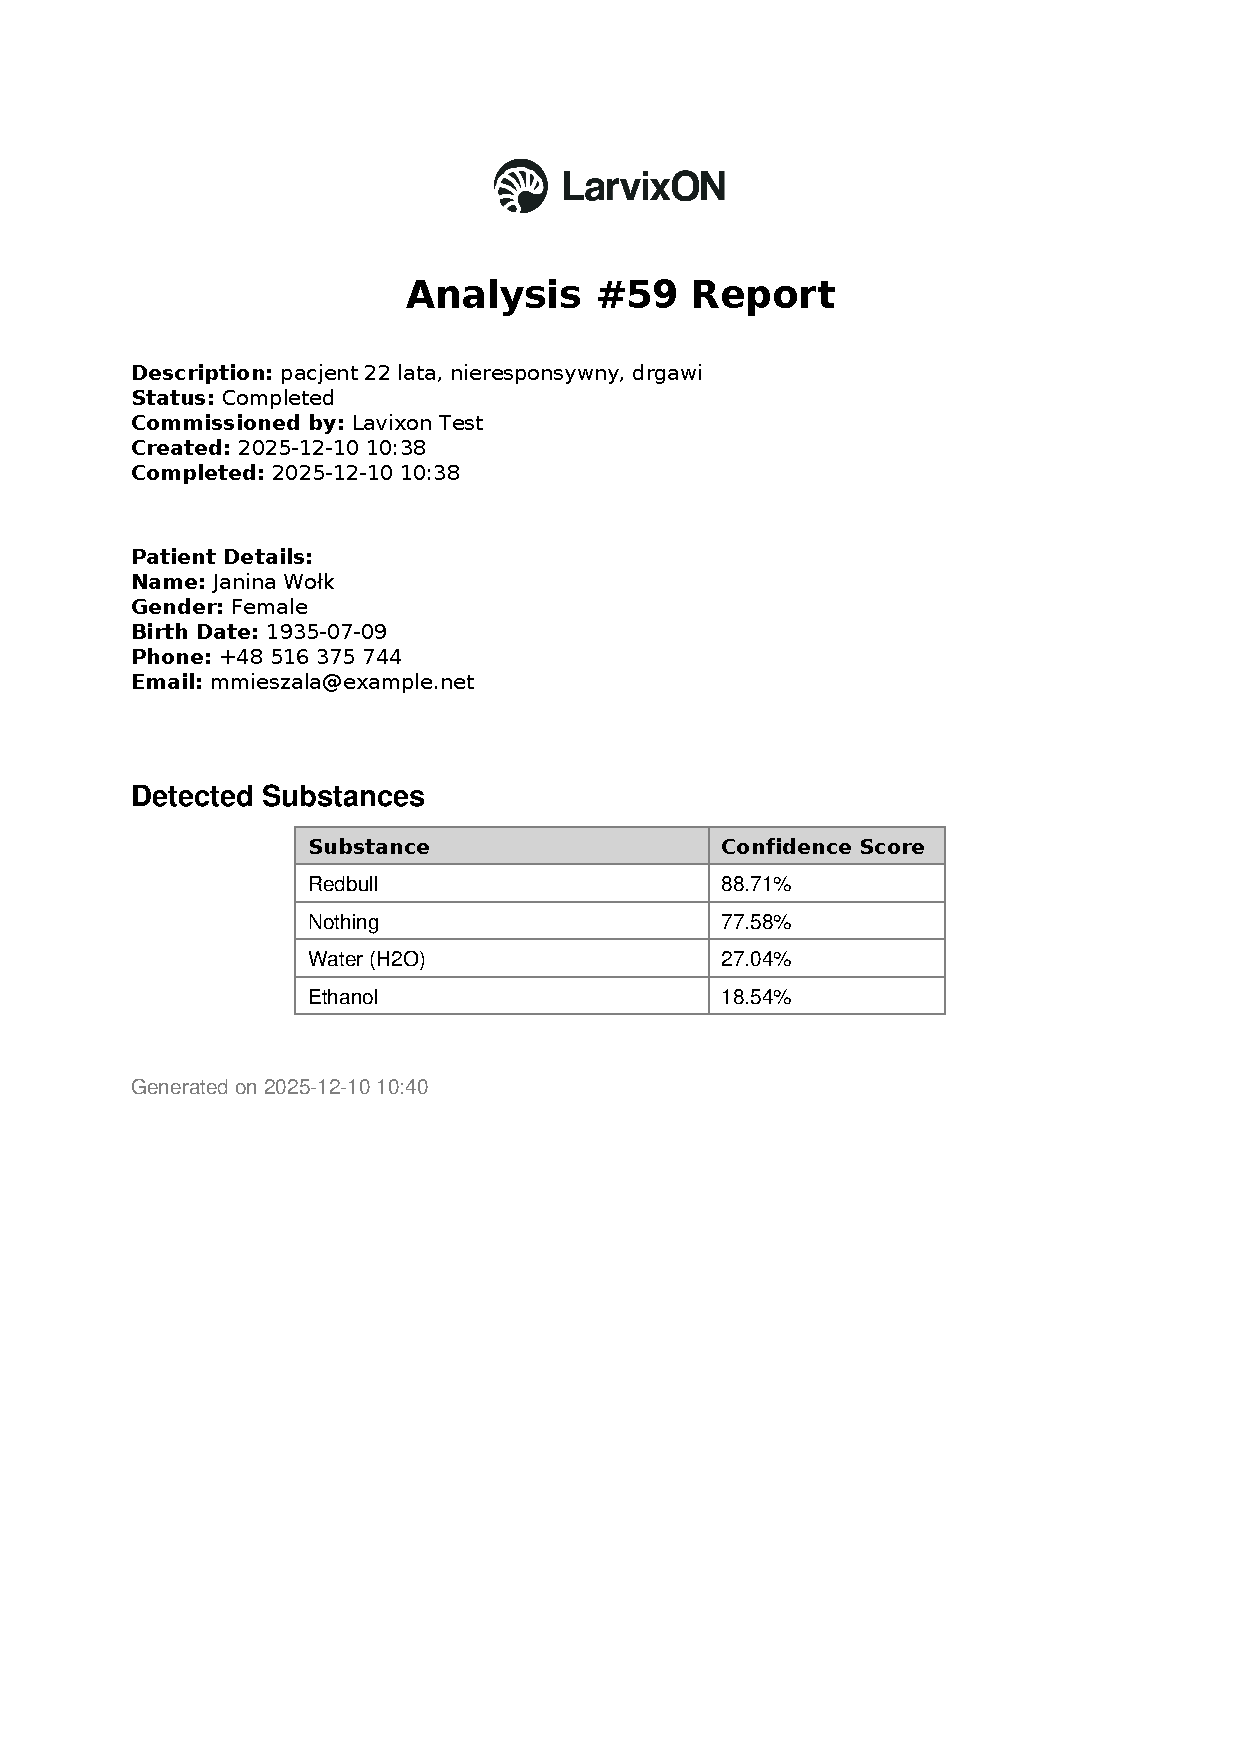
\includegraphics[width=1\textwidth]{images-frontend/app-ui/analysis_59_report.pdf}
    \caption{Wygenerowany raport}
    \label{fig:analysis_59_report}
\end{figure}

\paragraph{Moduł użytkownika\\}

Moduł użytkownika stanowi centrum zarządzania profilem w aplikacji. Główny widok został przedstawiony na rysunku ~\ref{fig:account}. W sekcji nagłówkowej wyeksponowano kluczowe dane identyfikacyjne, takie jak imię, nazwisko, adres e-mail oraz awatar. Poniżej umieszczono formularz edycyjny, pozwalający na aktualizację szczegółowych informacji: numeru telefonu, nazwy organizacji oraz biogramu (\ref{req:edit-profile}). Choć ostateczny układ interfejsu bazuje na pierwotnym prototypie (rys.~\ref{fig:mock-account}), wprowadzono w nim usprawnienia wizualne i funkcjonalne, w tym obsługę zdjęcia profilowego oraz przycisk umożliwiający wylogowanie z serwisu.

\begin{figure}[H]
    \centering
    \includegraphics[width=1\textwidth]{images-frontend/app-ui/account.png}
    \caption{Implementacja widoku konta użytkownika}
    \label{fig:account}
\end{figure}

\paragraph{Dodatkowe widoki\\}

\textbf{Polityka prywatności.}
Ze względu na wrażliwość danych przesyłanych do systemu, zdecydowano się wprowadzić widok Polityki Prywatności (rys.~\ref{fig:privacy-policy}). Realizuje on obowiązek informacyjny względem użytkowników, zgodnie z wymogami ochrony danych osobowych (RODO). Dokument ten prezentuje szczegółowy zakres zbieranych informacji, obejmujący m.in. dane konta czy sposób przetrzymywania przesyłanych nagrań.

\begin{figure}[H]
    \centering
    \includegraphics[width=1\textwidth]{images-frontend/app-ui/privacy-policy.png}
    \caption{Polityka prywatności}
    \label{fig:privacy-policy}
\end{figure}

\textbf{Regulamin korzystania z systemu.}
Sekcja Regulaminu (rys.~\ref{fig:rules}) definiuje zasady korzystania z platformy, kładąc szczególny nacisk na jej charakter badawczy i niekomercyjny. Użytkownik jest informowany, że aplikacja stanowi eksperymentalny prototyp rozwijany w ramach projektu akademickiego. Tekst reguluje kwestie związane z akceptacją warunków świadczenia usługi oraz opisuje główne funkcje systemu.

\begin{figure}[H]
    \centering
    \includegraphics[width=1\textwidth]{images-frontend/app-ui/rules.png}
    \caption{Regulamin}
    \label{fig:rules}
\end{figure}

\subsubsection{Obsługa błędów przy komunikacji z API}
W celu ujednolicenia mechanizmu detekcji i obsługi błędów w warstwie prezentacji, zastosowano wzorzec kreacyjny \textbf{Metoda wytwórcza}. Wprowadzono hierarchię klas, której podstawą jest abstrakcyjna klasa \textbf{Failure}. Pozwala ona w sposób jednoznaczny zidentyfikować przyczynę niepowodzenia operacji i podjąć odpowiednią akcję w interfejsie użytkownika (np. wyświetlenie komunikatu, wylogowanie użytkownika).

Błędy wynikające z komunikacji sieciowej zostały zgrupowane w klasie \textbf{ApiFailure}, dziedziczącej po \texttt{Failure}. Klasa ta przechowuje kod statusu HTTP, wiadomość dla użytkownika oraz opcjonalne, dedykowane pola. W celu dokładnej obsługi zdarzeń, zdefiniowano podklasy reprezentujące konkretne kategorie błędów. Przykładowe błędy:
\begin{itemize}
    \item \textbf{Błędy klienta (4xx)} (rys.\ref{fig:401failures}): BadRequestFailure (400), ValidationFailure (400 oraz wykryte błędy pól), UnauthorizedFailure (401) itp.
    \item \textbf{Błędy serwera (5xx)}: InternalServerErrorFailure (500), BadGatewayFailure (502) itp.
    \item \textbf{Nieznane błędy}: \texttt{UnknownApiFailure} (np. w przypadku braku kodu statusu).\end{itemize}

\begin{figure}[H]
    \centering
    \includegraphics[width=1\textwidth]{images-frontend/code/400failures.png}
    \caption{Przykładowe błędy 4xx}
    \label{fig:401failures}
\end{figure}

Bazowa klasa \texttt{ApiFailure} wykorzystuje konstruktor fabryczny (rys. \ref{fig:apifailure_factory}) zdefiniowany jako \texttt{factory ApiFailure.fromResponse}. Słowo kluczowe \textbf{factory} w języku Dart pozwala na to, aby konstruktor nie tworzył zawsze nowej instancji tej samej klasy, lecz mógł zwracać instancje klas pochodnych. Konstruktor ten przyjmuje jako argument obiekt typu \texttt{Response?} (gdzie znak „?” oznacza typ, który może również być typu null). Na podstawie kodu statusu HTTP zawartego w odpowiedzi, fabryka instancjonuje odpowiedni typ błędu domenowego.

\begin{figure}[H]
    \centering
    \includegraphics[width=1\textwidth]{images-frontend/code/apifailure_factory.png}
    \caption{Konstruktor fabryczny ApiFailure}
    \label{fig:apifailure_factory}
\end{figure}

W celu integracji z biblioteką klienta HTTP, wykorzystano mechanizm rozszerzeń, dostępny w języku Dart. Zaimplementowano rozszerzenie \textbf{ApiFailureMapperX} na klasie \textbf{DioException} (rys. \ref{fig:dio_extension}). Klasa \texttt{DioException} jest wyjątkiem zgłaszanym przez bibliotekę \texttt{dio} w momencie niepowodzenia żądania sieciowego. Dzięki zastosowaniu rozszerzenia, techniczny wyjątek biblioteki jest mapowany bezpośrednio na opisany wyżej domenowy obiekt \texttt{ApiFailure}, co pozwala na zachowanie czystości kodu.

\begin{figure}[H]
    \centering
    \includegraphics[width=1\textwidth]{images-frontend/code/dio_extension.png}
    \caption{Rozszerzenie klasy DioException}
    \label{fig:dio_extension}
\end{figure}

Tak przygotowany, otypowany obiekt błędu trafia następnie do warstwy zarządzania stanem (komponentu BLoC). Dzięki precyzyjnej hierarchii klas błędów, logika biznesowa może podjąć decyzję adekwatną do zaistniałej sytuacji. System może zareagować w sposób jawny, wyświetlając użytkownikowi komunikat, lub podjąć próbę ponowienia operacji bez zwracania uwagi użytkownika (np. przy chwilowej utracie połączenia).

\subsubsection{Zarządzanie stanem}
W celu zarządzania stanem aplikacji w warstwie prezentacji postanowiono wykorzystać popularną bibliotekę \texttt{flutter\_bloc}\footnote{Oficjalna dokumentacja biblioteki flutter\_bloc: \url{https://bloclibrary.dev/}}, która stanowi implementację wzorca BLoC (\textit{Business Logic Component}).

Wzorzec BLoC opiera się na reaktywnym paradygmacie programowania i wykorzystaniu strumieni. Przepływ danych (rys.\ref{fig:bloc_architecture}) odbywa się w następujący sposób: warstwa prezentacji emituje \textbf{zdarzenia}, które są przetwarzane przez BLoC, skutkując emisją nowego \textbf{stanu}, który wymusza odświeżenie wybranych widoków.

\begin{figure}[H]
    \centering
    \includegraphics[width=1\textwidth]{images-frontend/bloc_dataflow.png}
    \caption{Schemat przepływu danych w architekturze BLoC. Źródło: \cite{bloc-library}}
    \label{fig:bloc_architecture}
\end{figure}

\paragraph{Struktura stanu\\}
W projekcie przyjęto podejście oparte na pojedynczej, niemutowalnej klasie stanu, która agreguje wszystkie niezbędne dane dla danego widoku. Kluczowym elementem tej struktury jest:

\begin{itemize}
    \item \textbf{Status operacji} – zrealizowany za pomocą typu wyliczeniowego \texttt{enum} (np. \texttt{initial}, \texttt{loading}, \texttt{success}, \texttt{error}), który determinuje, co aktualnie dzieje się w obrębie danego komponentu.
    \item \textbf{Przechowywanie danych} – stan zawiera pola dla danych wynikowych oraz potencjalnych komunikatów błędów.
    \item \textbf{Niemutowalność i metoda \texttt{copyWith}} – ze względu na wymogi biblioteki BLoC, każda zmiana stanu  wiąże się z utworzeniem nowej instancji obiektu stanu. W tym celu zaimplementowano metodę \texttt{copyWith}, która pozwala na skopiowanie obecnego stanu z nadpisaniem tylko wybranych pól.
\end{itemize}

\paragraph{Optymalizacja odświeżania widoku\\}
Aby zapobiec zbędnym przebudowom interfejsu, klasa stanu rozszerza bibliotekę \textbf{Equatable}\footnote{Oficjalna dokumentacja biblioteki equatable: \url{https://pub.dev/documentation/equatable/latest/}}. Pozwala ona na porównywanie obiektów przez wartość, a nie przez referencję. Dzięki temu, jeśli nowa instancja stanu zawiera identyczne dane co poprzednia, mechanizm BLoC nie wymusi odświeżenia komponentów prezentacji, co pozytywnie wpływa na wydajność aplikacji.

\paragraph{Przykład - moduł ustawień\\}

Jako przykład zastosowania zarządzania stanem wybrano moduł ustawień. Pozwala on użytkownikowi na modyfikację preferencji, takich jak język interfejsu czy motyw (jasny/ciemny).

Za logikę biznesową odpowiada w tym przypadku klasa \texttt{SettingsCubit} (będąca uproszczoną wersją BLoC, rys.\ref{fig:settings_cubit}), która operuje na stanie \texttt{SettingsState} (rys. \ref{fig:settings_state}). Stan ten przechowuje dwie kluczowe informacje:
\begin{itemize}
    \item \texttt{theme}: aktualnie wybrany tryb wyświetlania,
    \item \texttt{locale}: aktualnie wybrany język aplikacji.
\end{itemize}

\begin{figure}[H]
    \centering
    \includegraphics[width=1\textwidth]{images-frontend/code/settings_state.png}
    \caption{Definicja klasy stanu SettingsState}
    \label{fig:settings_state}
\end{figure}

Przepływ sterowania w przypadku zmiany motywu wygląda następująco:

\begin{enumerate}
    \item Użytkownik w widoku ustawień wybiera nowy motyw. Skutkuje to wywołaniem metody \texttt{setTheme} w  \texttt{SettingsCubit}.
    \item Metoda ta komunikuje się z warstwą repozytorium, aby trwale zapisać wybór użytkownika w pamięci urządzenia.
    \item Po poprawnym zapisie, Cubit emituje nową instancję stanu metodą \texttt{emit(..)}.
\end{enumerate}

\begin{figure}[H]
    \centering
    \includegraphics[width=1\textwidth]{images-frontend/code/settings_cubit.png}
    \caption{Fragment definicji klasy SettingsCubit}
    \label{fig:settings_cubit}
\end{figure}

Reakcja interfejsu jest natychmiastowa dzięki zastosowaniu widgetu \texttt{BlocBuilder}, który nasłuchuje na zmiany stanu podanego komponentu BLoC, na najwyższym poziomie drzewa widgetów. Jak przedstawiono na rys. \ref{fig:settings_main}, każda emisja nowego stanu powoduje przebudowanie głównego widgetu aplikacji z nowymi parametrami \texttt{themeMode} oraz \texttt{locale}, co dynamicznie zmienia wygląd całej aplikacji.

\begin{figure}[H]
    \centering
    \includegraphics[width=1\textwidth]{images-frontend/code/settings_main.png}
    \caption{Wykorzystanie stanu ustawień do zmiany preferencji na najwyższym poziomie aplikacji}
    \label{fig:settings_main}
\end{figure}

\subsubsection{Automatyczna dokumentacja kodu}
W ekosystemie języka Dart standardem jest wykorzystanie narzędzia \texttt{dartdoc}\footnote{Oficjalna dokumentacja narzędzia dartdoc: \url{https://dart.dev/tools/dart-doc}}, które umożliwia automatyczne generowanie dokumentacji API bezpośrednio z kodu źródłowego.

Kluczowym elementem są tutaj tzw. \textit{komentarze dokumentujące}, oznaczane w składni języka za pomocą potrójnego ukośnika (\texttt{///}). Pozwalają one na opisywanie klas, metod oraz zmiennych z wykorzystaniem formatowania \textbf{Markdown}. Dzięki temu możliwe jest nie tylko dodawanie opisów tekstowych, ale również:
\begin{itemize}
    \item tworzenie list i tabel,
    \item umieszczanie fragmentów przykładowego kodu,
    \item tworzenie aktywnych odnośników do innych elementów kodu (poprzez ujęcie nazwy klasy lub metody w nawiasy kwadratowe, np. \texttt{[ApiFailure]}).
\end{itemize}

Wynikiem działania narzędzia jest zestaw statycznych plików HTML, prezentujący strukturę projektu w czytelnej formie. Przykład został przedstawiony na rysunku \ref{fig:frontend_documentation}.

\begin{figure}[H]
    \centering
    \includegraphics[width=1\textwidth]{images-frontend/code/dokumentacja.png}
    \caption{Dokumentacja klasy \texttt{Analysis}}
    \label{fig:frontend_documentation}
\end{figure}

\subsubsection{Testy akceptacyjne i z udziałem użytkowników}

Celem testów z udziałem użytkowników była weryfikacja użyteczności interfejsu oraz potwierdzenie, że zaimplementowane funkcjonalności pokrywają zdefiniowane wymagania biznesowe.

Testy przeprowadzono w oparciu o przygotowane scenariusze testowe, odwzorowujące typowe ścieżki postępowania użytkownika w systemie. W testach aktywnie brali udział członkowie zespołu deweloperskiego oraz (sporadycznie) interesariusze.

Szczególną uwagę zwrócono na:
\begin{itemize}
    \item \textbf{Intuicyjność nawigacji} – czy użytkownik potrafi samodzielnie poruszać się po aplikacji bez uprzedniego szkolenia.
    \item \textbf{Obsługę błędów} – czy system czytelnie komunikuje napotkane problemy.
    \item \textbf{Responsywność} – weryfikacja czytelności interfejsu na urządzeniach mobilnych oraz desktopowych.
\end{itemize}

Poniższa tabela (tab. \ref{tab:test_scenarios}) prezentuje przykładowe scenariusze testowe, które zostały poddane weryfikacji manualnej.

\begin{longtable}{|p{0.18\textwidth}|p{0.35\textwidth}|p{0.35\textwidth}|p{0.1\textwidth}|}
    \hline
    \textbf{ID Scenariusza} & \textbf{Opis czynności}                                                        & \textbf{Oczekiwany rezultat}                                                                              \\ \hline
    \endhead

    TC-01                   & Rejestracja nowego użytkownika z podaniem niepoprawnego formatu adresu e-mail. & System blokuje wysyłkę formularza i wyświetla komunikat walidacji pod odpowiednim polem.                  \\ \hline

    TC-02                   & Logowanie przy użyciu poprawnych danych uwierzytelniających.                   & Użytkownik zostaje przekierowany do widoku listy analiz.                                                  \\ \hline

    TC-03                   & Przesłanie pliku wideo w formacie o dopuszczonym rozmiarze (<3 GB).            & Plik zostaje przesłany, pojawia się pasek postępu, a następnie analiza zmienia status na "Przetwarzanie". \\ \hline

    TC-04                   & Odczyt wyników analizy i generowanie raportu PDF.                              & Wyświetlają się wykryte toksyny. Po kliknięciu "Eksportuj" generowany jest plik zgodny z szablonem.       \\ \hline
    \caption{Zestawienie wybranych manualnych scenariuszy testowych}
    \label{tab:test_scenarios}
\end{longtable}

Przeprowadzone testy manualne pozwoliły na wykrycie i wyeliminowanie szeregu błędów interfejsu na wczesnym etapie prac. Najważniejsze poprawki wdrożone na podstawie informacji zwrotnej od testerów to:
\begin{enumerate}
    \item \textbf{Rozdzielenie procesu zlecania analizy na kroki:} Pierwotnie formularz znajdował się na jednym długim ekranie, co testerzy uznali za przytłaczające. Wprowadzono "Kreator analizy".
    \item \textbf{Wskaźniki ładowania:} Dodano ekrany szkieletowe m.in. przy pobieraniu szczegółów analizy, ponieważ użytkownicy nie mieli pewności, czy aplikacja się zawiesiła, czy pobiera dane.
    \item \textbf{Komunikaty błędów:} Zastąpiono techniczne kody błędów API (np. "500 Internal Server Error") czytelnymi dla człowieka komunikatami (np. "Wystąpił problem z serwerem, spróbuj ponownie później").
\end{enumerate}

Ostateczna wersja systemu przeszła pomyślnie testy akceptacyjne, realizując założone wymagania funkcjonalne.

\subsection{Implementacja modelu uczenia maszynowego (Larvixon ML)}
\label{ssec:ml-implementation}

\noindent Implementacja modelu $ML$ (PyTorch) była zorientowana na wydajne przetwarzanie czasowo-przestrzenne danych wideo i zapewnienie środowiska gotowego do serwowania predykcji.

\subsubsection{Architektura Modelu i Warstwy}
\label{sssec:ml-architecture-layers}

\noindent Wybrano architekturę hybrydową \textbf{CNN+LSTM} zoptymalizowaną do klasyfikacji krótkich sekwencji wideo.

\begin{enumerate}
    \item \textbf{Warstwa Ekstrakcji Cech (CNN):}
          \begin{itemize}
              \item Wykorzystano gotową, wstępnie wytrenowaną architekturę \textbf{ResNet18} (dostępną w PyTorch), co znacząco przyspieszyło zbieżność i zmniejszyło wymaganą ilość danych treningowych.
              \item Ostatnie warstwy klasyfikacyjne sieci \textit{ResNet18} zostały usunięte. Rolą \textit{CNN} jest działanie jako \textbf{extractor cech}, redukujący każdą klatkę o wymiarach $[3, 112, 112]$ do wektora cech wysokiego poziomu (tzw. \textit{embedding}).
          \end{itemize}
    \item \textbf{Warstwa Modelowania Czasowego (LSTM):}
          \begin{itemize}
              \item Wektory cech, sekwencyjnie generowane przez warstwę \textit{CNN}, są podawane do sieci \textbf{LSTM} (Long Short-Term Memory).
              \item \textit{LSTM} skutecznie uczy się zależności i dynamiki czasowej, tj. w jaki sposób ewolucja wzorców ruchu (modyfikowanych przez \textit{CurrentMovementModifier} w symulacji) koreluje z klasą substancji.
          \end{itemize}
    \item \textbf{Warstwa Klasyfikacyjna (Fully Connected):}
          \begin{itemize}
              \item Finalny wektor stanu z \textit{LSTM} jest przekazywany przez warstwy gęste (FC), które mapują cechy behawioralne na zdefiniowaną przestrzeń klas (substancji).
              \item Na wyjściu stosowana jest funkcja aktywacji \textit{softmax} do generowania rozkładu prawdopodobieństwa predykcji.
          \end{itemize}
\end{enumerate}

\subsubsection{Trening, Walidacja i Wnioskowanie}
\label{sssec:ml-training-inference}

\noindent Faza implementacji obejmowała kluczowe aspekty związane z zarządzaniem danymi i środowiskiem.

\begin{itemize}
    \item \textbf{Zbiór Danych:} W początkowej fazie wykorzystano dane wygenerowane przez \textbf{Larvixon Simulation}. Dzięki precyzyjnemu modelowaniu modyfikatorów ruchu (\textit{np. SpeedMultiplier}, \textit{RandomnessMultiplier}) oraz ich dynamiki czasowej (\textit{onsetTime}, \textit{duration}, \textit{comedownTime}), dane syntetyczne miały wysoką wartość wczesnowalidacyjną dla architektury.
    \item \textbf{Funkcja Straty:} Zastosowano \textbf{Cross-Entropy Loss} jako funkcję straty dla problemu klasyfikacji wieloklasowej.
    \item \textbf{Wnioskowanie (\textit{Inference}):} Moduł \textit{ML} został skonteneryzowany (\textbf{Docker}) wraz z zależnościami \textit{PyTorch}. Wnioskowanie jest serwowane za pośrednictwem dedykowanego API opartego na \textbf{FastAPI}, co zapewnia minimalne opóźnienia i wysoką przepustowość.
    \item \textbf{Walidacja:} Proces implementacji był ściśle konsultowany z dr Piórkowską w celu walidacji podejścia, prawidłowości implementacji modelu oraz badania jego celności na danych spoza treningowego zbioru danych, co przyczyniło się do osiągnięcia stabilnej dokładności w zakresie 60\
\end{itemize}

\subsection{Implementacja symulacji}

\subsubsection{Algorytm fizycznego ruchu larw}

Nietrywialnym algorytmem jest sposób poruszania się larw w symulacji. Każda larwa to tak naprawdę 5 punktów, gdzie punkt nr 1 odpowiada jej głowie, a punkt nr 5 jej odwłokowi (reszta po kolei między tymi punktami). Dla każdej pary sąsiadujących punktów jest zdefiniowana preferowana odległość, która może się zmieniać. Ruch larwy składa się z trzech faz:

\begin{enumerate}
    \item Zwiększenie preferowanej odległości między punktami 1. a 2. Oznacza to, że głowa larwy podróżuje do przodu.
    \item Reset preferowanej odległości między punktami 1. a 2. oraz zmniejszenie preferowanej odległości między punktami 4. i 5. Oznacza to, że odwłok larwy przybliża się do reszty ciała.
    \item Reset wszystkich preferowanych odległości. Oznacza to, że przez 1/3 czasu punkty larwy dążą do pozycji, jakby była w spoczynku.
\end{enumerate}

Po wyliczeniu w danej fazie preferowanej odległości, w każdej klatce do czasu następnej fazy logika obsługująca fizykę zwiększa przyspieszenie punktów tak, aby znalazły się w preferowanych odległościach do sąsiadów. Na przykład w fazie pierwszej, dzięki wzajemnym oddziaływaniom punktów na siebie, punkt 1. jest bardziej popychany do przodu niż punkt 2. do tyłu, a to dlatego, że punkt 2. ma za sobą 3 inne punkty, które ciężej mu “popchnąć”.

Na ruch larw wpływają narkotyki - dla larwy wyliczany jest jej \textit{CurrentMovementModifier}. Algorytm jego wyliczenia jest opisany w sekcji \ref{sec:modifieralgorithm}. \textit{MovementModifier} posiada następujące parametry:
\begin{enumerate}
    \item \textbf{SpeedMultiplier} - wpływa głównie na zwiększanie prędkości larwy
    \item \textbf{SegmentCoordinationMultiplier} - wpływa głównie na wzmocnienie/osłabienie efektów wynikajacych z faz larwy
    \item \textbf{RandomnessMultiplier} - wpływa głównie na ciągłe zmienianie kierunku głowy larwy
    \item \textbf{DirectionStability} - wpływa na możliwość mocniejszej zmiany kierunku i zmienia losowo pozycję punktu, do którego larwa dąży na nieco inny
    \item \textbf{SegmentSyncMultiplier} - może sprawić, że następna faza ruchu zostanie wybrana losowo
    \item \textbf{HeadForceMultiplier} - wpływa na to, z jaką siłą larwa dąży do wybranego kierunku
    \item \textbf{RestoreForceMultiplier} - wpływa na to, z jaką siłą wszystkie punkty kierują się w swoje preferowane kierunki
\end{enumerate}

\subsubsection{Wyliczenie wartości modyfikatorów narkotyków}
\label{sec:modifieralgorithm}
Dla zwiększenia realistyczności, narkotyki nie działają od razu. Narkotyki aplikowane są z określonym \textit{Intensity}, które rośnie z 0 do podanego celu. Dodatkowo narkotyki mają parametry:
\begin{enumerate}
    \item \textbf{onsetTime}, który definiuje czas etapu zwiększania \textit{intensity}.
    \item \textbf{duration}, który definiuje czas etapu utrzymania \textit{intensity}.
    \item \textbf{comedownTime}, który definiuje czas etapu zmniejszania \textit{intensity} do 0 (jeśli larwa dożyje ostatniej fazy).
\end{enumerate}
Dzięki wykorzystaniu wzorca projektowego \textit{NullObject} do opisu parametrów ruchu dla larwy w domyślnym stanie (\textit{MovementModifier.Normal}), wyliczenie finalnego modyfikatora ruchu larwy polega na liniowej interpolacji między \textit{MovementModifier.Normal} i wszystkimi \textit{MovementModifier} wyliczonymi dla narkotyków na podstawie ich intensywności.

\section{Demonstracja produktu programowego}

\subsection{Przykładowy workflow wykonywania analizy}
W celu zaprezentowania kluczowych funkcjonalności systemu, poniżej przedstawiono kompletny scenariusz realizacji zadania diagnostycznego przez zalogowanego użytkownika. Proces ten obejmuje autoryzację, zlecenie analizy wideo, monitorowanie jej statusu oraz interpretację otrzymanych wyników.

\subsubsection*{Krok 1: Autoryzacja i dostęp do systemu}
Proces rozpoczyna się na ekranie powitalnym (rys.~\ref{fig:landing}), skąd użytkownik przechodzi do panelu logowania. Po wprowadzeniu poprawnych danych uwierzytelniających następuje przekierowanie do głównego widoku aplikacji. W przypadku nowych użytkowników dostępna jest ścieżka rejestracji.

\paragraph*{Scenariusz alternatywny}
Jeżeli użytkownik korzystał już wcześniej z aplikacji, system automatycznie weryfikuje ważność przechowywanego lokalnie tokenu dostępu. W przypadku pozytywnej walidacji sesji, etap wprowadzania danych logowania jest pomijany, a użytkownik uzyskuje natychmiastowy dostęp do panelu analiz.

\subsubsection*{Krok 2: Zlecenie nowej analizy}
Użytkownik inicjuje proces badawczy, wybierając opcję dodania nowej analizy. Uruchamia to wieloetapowy kreator (rys.~\ref{fig:new-analysis}), który prowadzi użytkownika przez proces konfiguracji badania:
\begin{enumerate}
    \item \textbf{Przesłanie materiału wideo:} Użytkownik wgrywa plik z nagraniem larw.
    \item \textbf{(opcjonalne) Wprowadzenie opisu klinicznego:} Użytkownik wprowadza opis przypadku klinicznego.
    \item \textbf{(opcjonalne) Powiązanie z pacjentem:} W kolejnym kroku następuje identyfikacja pacjenta. Dzięki zintegrowanej wyszukiwarce (rys.~\ref{fig:analysis-add-2}) użytkownik może odnaleźć kartotekę pacjenta po numerze PESEL, bez konieczności ręcznego przepisywania danych osobowych.
\end{enumerate}

\begin{figure}[H]
    \centering
    \includegraphics[width=0.5\linewidth]{new_analysis.png}
    \caption{Widok ekranu kreatora nowej analizy}
    \label{fig:new-analysis}
\end{figure}

\subsubsection*{Krok 3: Monitorowanie postępu}
Po zatwierdzeniu formularza, nowe zlecenie pojawia się na liście analiz (rys.~\ref{fig:analyses-grid-filter-processing}). Użytkownik ma możliwość śledzenia statusu przetwarzania (np. \textit{Oczekujące}, \textit{Przetwarzanie}, \textit{Zakończono})

\begin{figure}[H]
    \centering
    \includegraphics[width=0.5\linewidth]{grid_waiting_for_result.png}
    \caption{Widok gridu analiz, wraz z nową analizą oczekującą na przetworzenie}
    \label{fig:analyses-grid-filter-processing}
\end{figure}

\subsubsection*{Krok 4: Odczyt wyników i raportowanie}
Po zakończeniu przetwarzania, użytkownik uzyskuje dostęp do szczegółowych wyników. Widok ten prezentuje:
\begin{itemize}
    \item Grafikę będącą miniaturką nagrania (rys.~\ref{fig:redbull_miniature}).
    \item Metadane dot. analizy, takie jak data zlecenia, status, informacje o pacjencie, opis kliniczny (rys.~\ref{fig:redbull_miniature}).
    \item Wykryte substancje toksyczne wraz ze wskaźnikami pewności predykcji (rys.~\ref{fig:results_redbull})
\end{itemize}
Umożliwia to podjęcie decyzji medycznej w oparciu o dostarczone dane. Opcjonalnie użytkownik może wygenerować sformalizowany raport (rys.~\ref{fig:dr_mikolaj}), który może zostać dołączony do zewnętrznej dokumentacji medycznej pacjenta.

\begin{figure}[H]
    \centering
    \includegraphics[width=0.5\linewidth]{redbull_miniature.png}
    \caption{Widok tytułu analizy, miniaturki, danych pacjenta}
    \label{fig:redbull_miniature}
\end{figure}

\begin{figure}[H]
    \centering
    \includegraphics[width=0.5\linewidth]{results_redbull.png}
    \caption{Widok rezultatu obliczonego przez model maszynowy}
    \label{fig:results_redbull}
\end{figure}

\begin{figure}[H]
    \centering
    \includegraphics[width=0.5\linewidth]{dr_mikolaj.png}
    \caption{Wyeksportowany raport z analizy}
    \label{fig:dr_mikolaj}
\end{figure}

\clearpage

\section{Dodatkowe materiały online}

\begin{enumerate}
    \item \href{https://github.com/orgs/LarvixON-ZPI/projects/1/views/1?filterQuery=}{nasz board w GitHub Projects}
    \item \href{https://github.com/LarvixON-ZPI/larvixon-backend}{larvixon-backend}
    \item \href{https://github.com/LarvixON-ZPI/larvixon-frontend}{larvixon-frontend}
    \item \href{https://github.com/LarvixON-ZPI/larvixon-model}{larvixon-model}
    \item \href{https://github.com/LarvixON-ZPI/larvixon-patients-service}{larvixon-patients-service}
    \item \href{https://github.com/LarvixON-ZPI/larvixon-simulation}{larvixon-simulation}
    \item \href{https://github.com/LarvixON-ZPI/larvixon-documentation}{larvixon-documentation}
\end{enumerate}

\clearpage
\nocite{*}
\printbibliography

\end{document}